\section{Asymmetry Extraction}
 %Now that we have discussed our selection criteria for charged pions and $\pi^0$ and $\eta$ mesons, t
 
 This section reviews the extraction of Collins asymmetries from the data sample passing all selection criteria discussed in the previous section.
 %Fig.~\ref{fig:pipiP0phi} shows examples of the Collins angle $\phi_1+\phi_2$ of $\pi^0\pi^+$ pairs. 
As discussed in Section~\ref{sec:observable}, we use the double-ratio method to cancel effects of non-uniform acceptance effects.
Remaining so-called false asymmetries are estimated from simulation and discussed in Section~\ref{sec:resutlsfrommc}. 
They will be used to correct the experimental asymmetry.  Their uncertainties are propagated to the systematic uncertainties.
The results from experimental data are discussed in Section~\ref{sec:resultsfromexp}.

\subsection{Results from Simulation}
\label{sec:resutlsfrommc}
Before moving to asymmetry measurement for the experimental data, we test the residual asymmetries caused by the acceptance using  Monte Carlo data. The Monte Carlo does not contain a Collins effect  so the double ratio asymmetry measured in the signal window should be 0. However, the detector acceptance may generate a dependence of the data on the azimuthal angle $\phi_{12}$ similar to the dependence caused by the Collins effect to be measured, as shown in Fig.~\ref{fig:differentthetarange} (note that  Fig.~\ref{fig:differentthetarange} shows the asymmetry before the application of the double ratio), and leads to false asymmetries. The previously introduced fiducial cuts make this effect smaller but  not to disappear.
This illustrates the need for the double-ratio method, which almost cancels entirely the false asymmetry. Any remaining effect 
is used to correct the experimental asymmetry and the statistical uncertainty of that correction is propagated to the systematic uncertainties.

\begin{figure}[b]
    \centering
    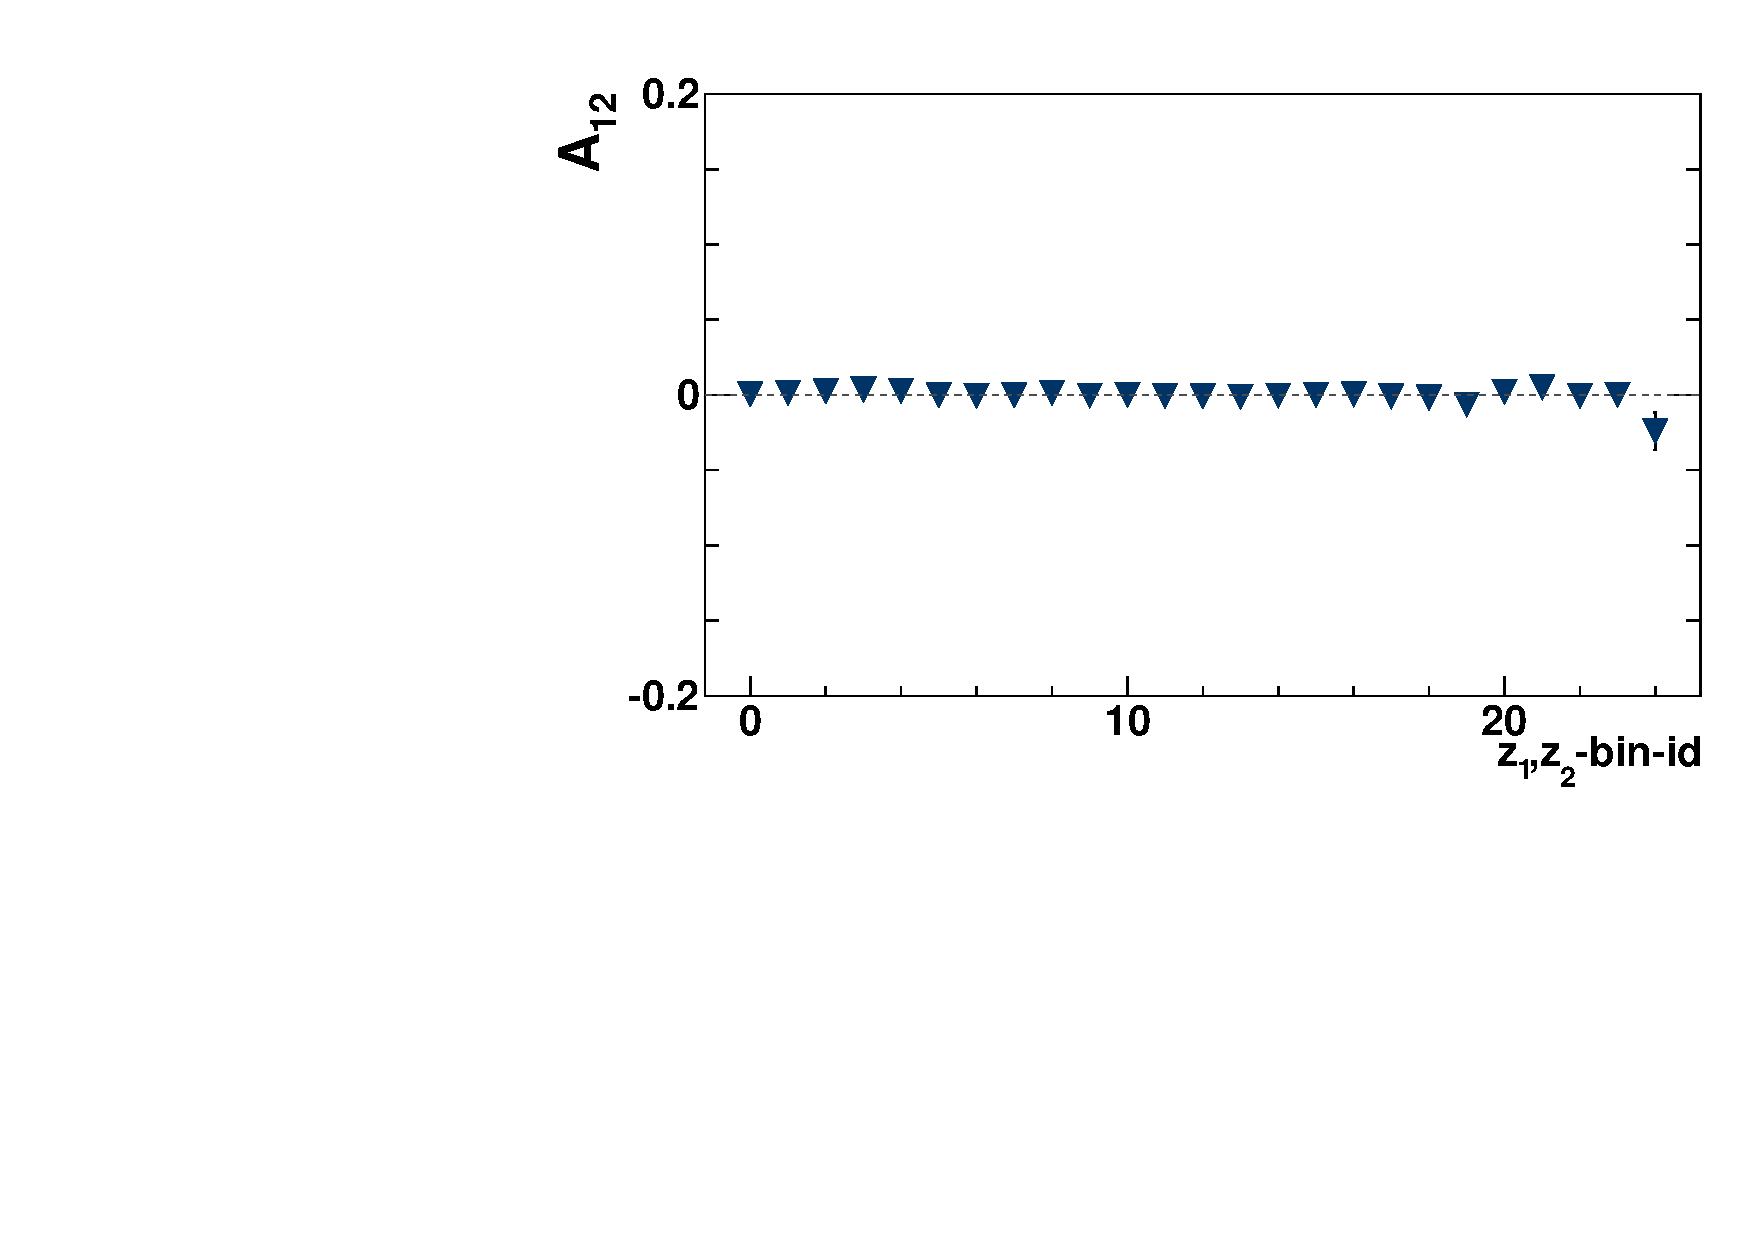
\includegraphics[width=0.6\textwidth,natwidth=250,natheight=100]{figure_asy/ComZ_Phi12_pi0.pdf}
    \caption{Asymmetry $A_{12}^{\pi^0}$ in  $(z_1,z_{2})$ bins measured with simulated data.}
    \label{fig:mc_example}
\end{figure}

As an example, the $A_{12}^{\pi^{0}}$ results of the relevant cosine fit to the $R_{12}^{\pi^0}\equiv R_{12}^{0\pm}/R_{12}^L$ double ratio in simulation is shown in Fig.~\ref{fig:mc_example}. 
This asymmetry can be determined with higher precision than $A_{12}^{\eta}$ and demonstrates that the remaining false asymmetries are small (detailed results on all false asymmetry can be found in the supporting spreadsheet summarized in Appendix~\ref{sec:spreadsheet}).



%For the final result we correct the asymmetry measured in the experimental data with the false asymmetry obtained from MC and the uncertainty on the false asymmetry will contribute to the systematic uncertainties.

\subsection{Results from Experimental Data}
\label{sec:resultsfromexp}
\subsubsection{\texorpdfstring{Raw Asymmetry of $\pi^0$ and $\eta$}{Raw Asymmetry of pi0 and eta}}
Data used in this study encompass Belle experiments  7 to 73.
Figure~\ref{fig:exp_pi0_result} shows  $A_{12}^{\pi^0}$ results for the $z_1$, $P_{t1}$, $(z_1,z_2)$, and $(P_{t1},P_{t2})$ binning. We call these asymmetries `raw' asymmetries, since they have not been corrected for smearing effects or for false asymmetries. 
In the binnings that are only differential in one variable, we observe significant asymmetries that rise with $z$ and $P_{t}$. This is consistent with the previous results for charged pions~\cite{ChargedPionResult2, ChargedPionResult}.

\begin{figure}[t]
  \centering     
    \subfigure[$\pi^0$ $z_1$ bins asymmetry]{\label{fig:exp_singlez}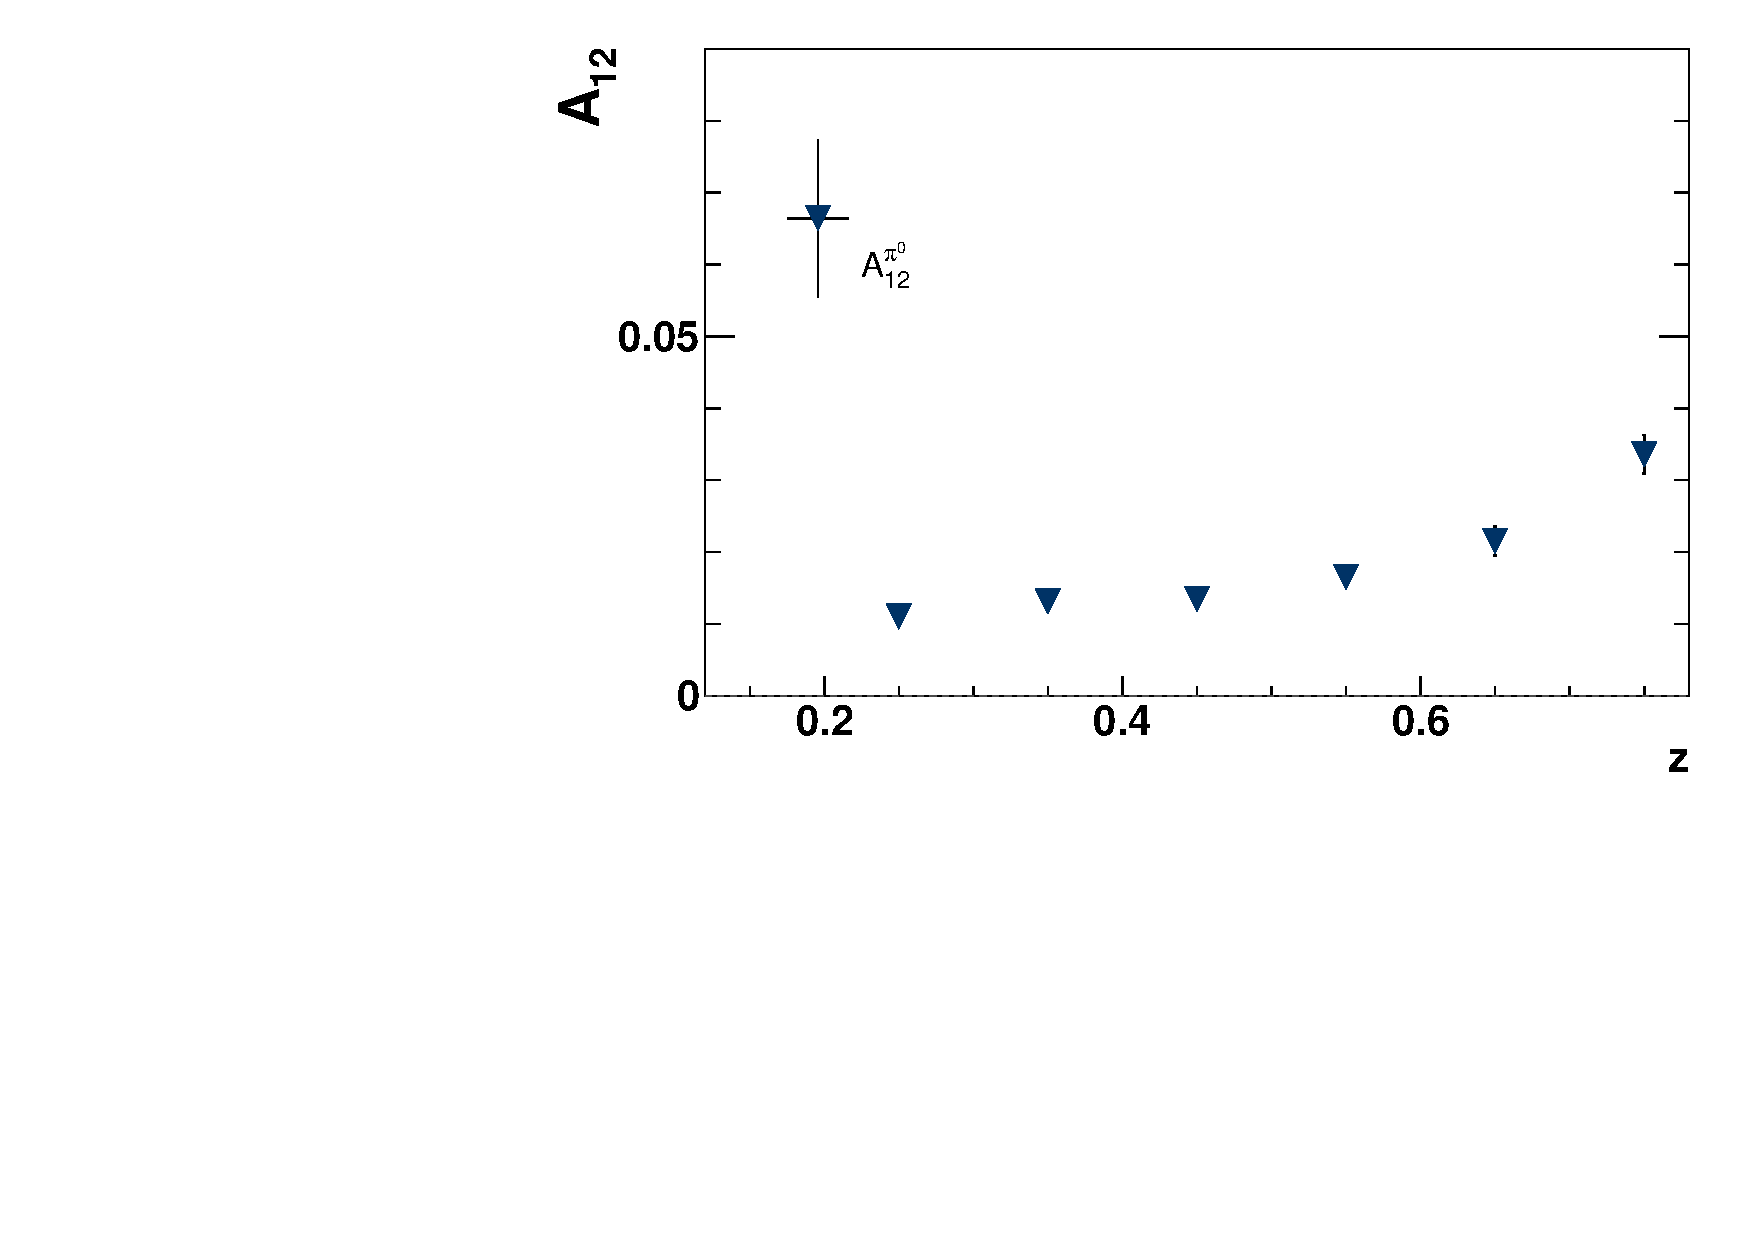
\includegraphics[width=.49\textwidth,natwidth=800,natheight=600]{figure_asy/Pi0NoCorrection0.pdf}}
 \subfigure[$\pi^0$ $P_{t1}$ bins asymmetry]{\label{fig:exp_singlez1}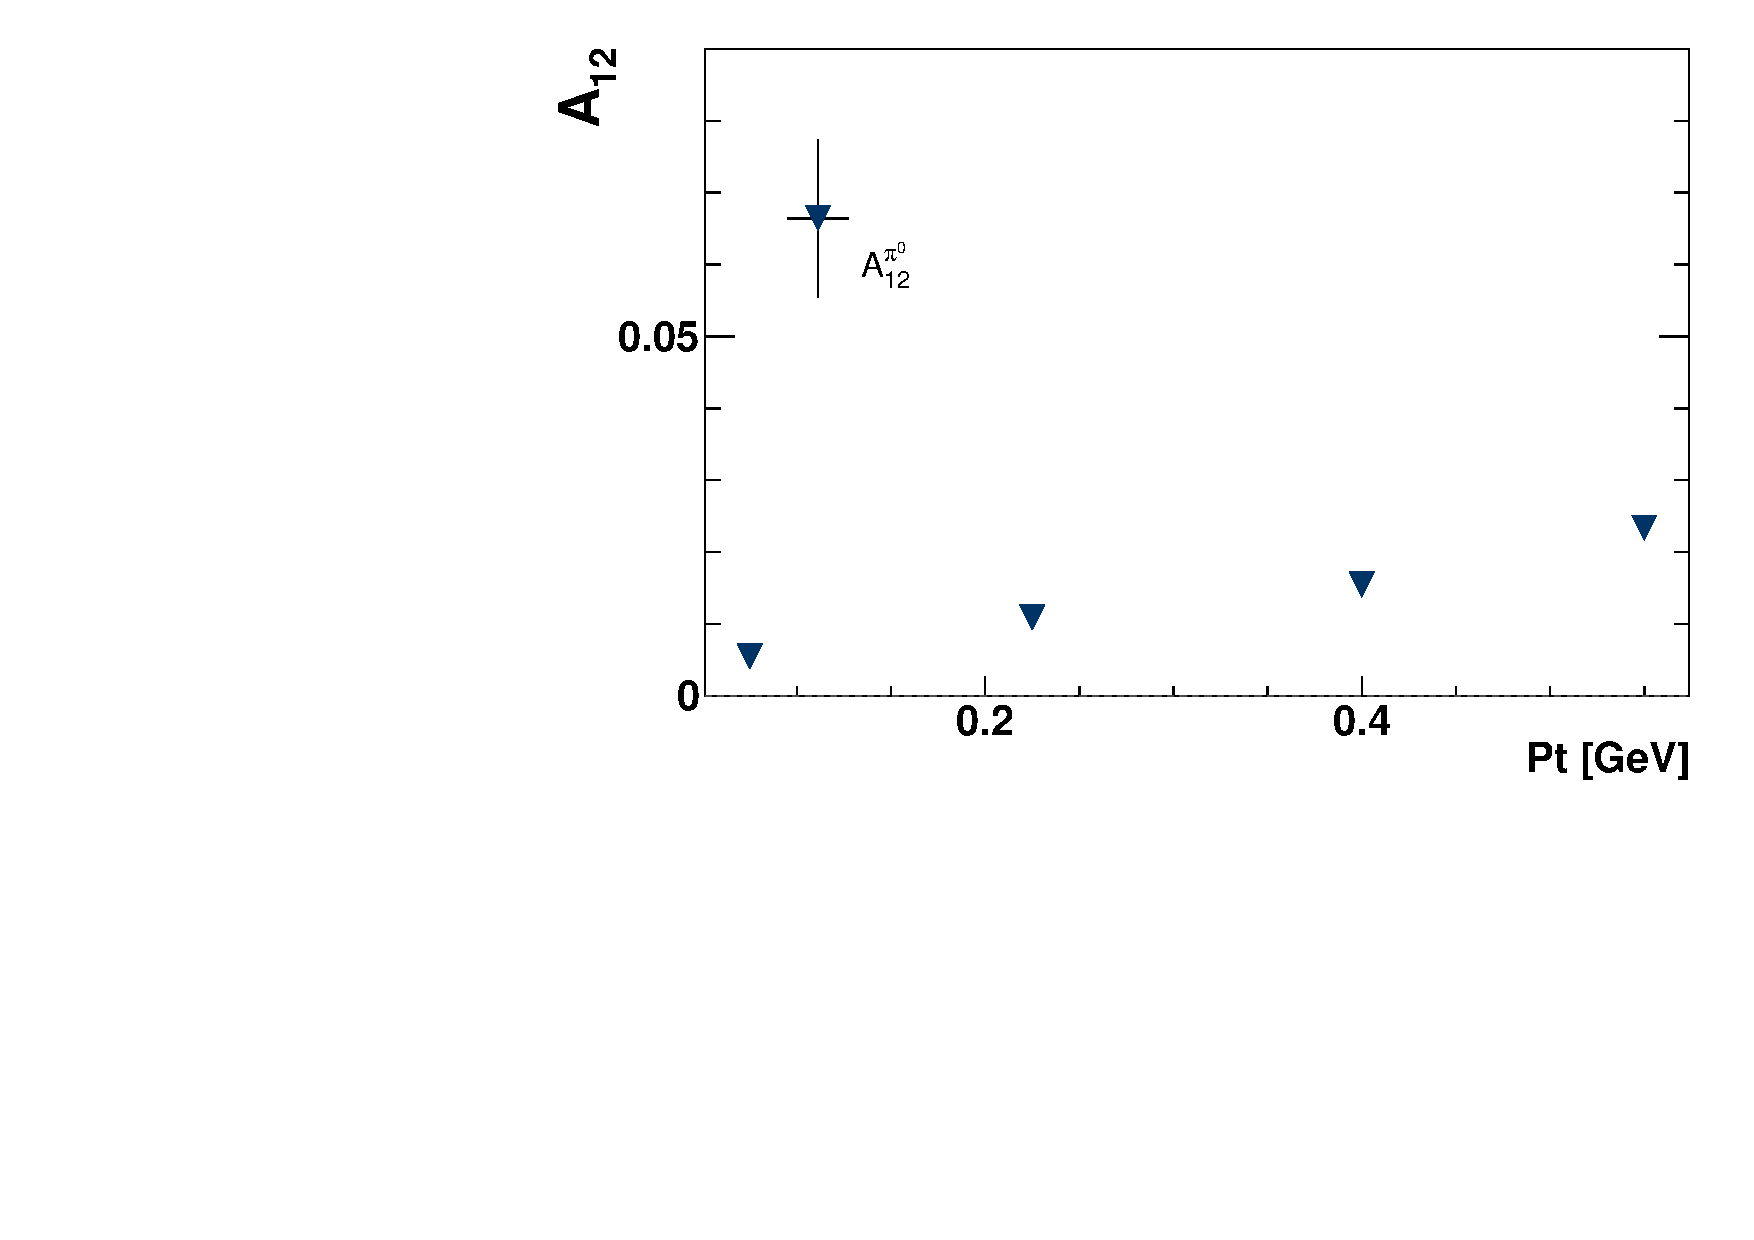
\includegraphics[width=.49\textwidth,natwidth=800,natheight=600]{figure_asy/Pi0NoCorrection2.pdf}}
  \subfigure[$\pi^0$ $(z_1,z_2)$ bins asymmetry]{\label{fig:exp_singlept}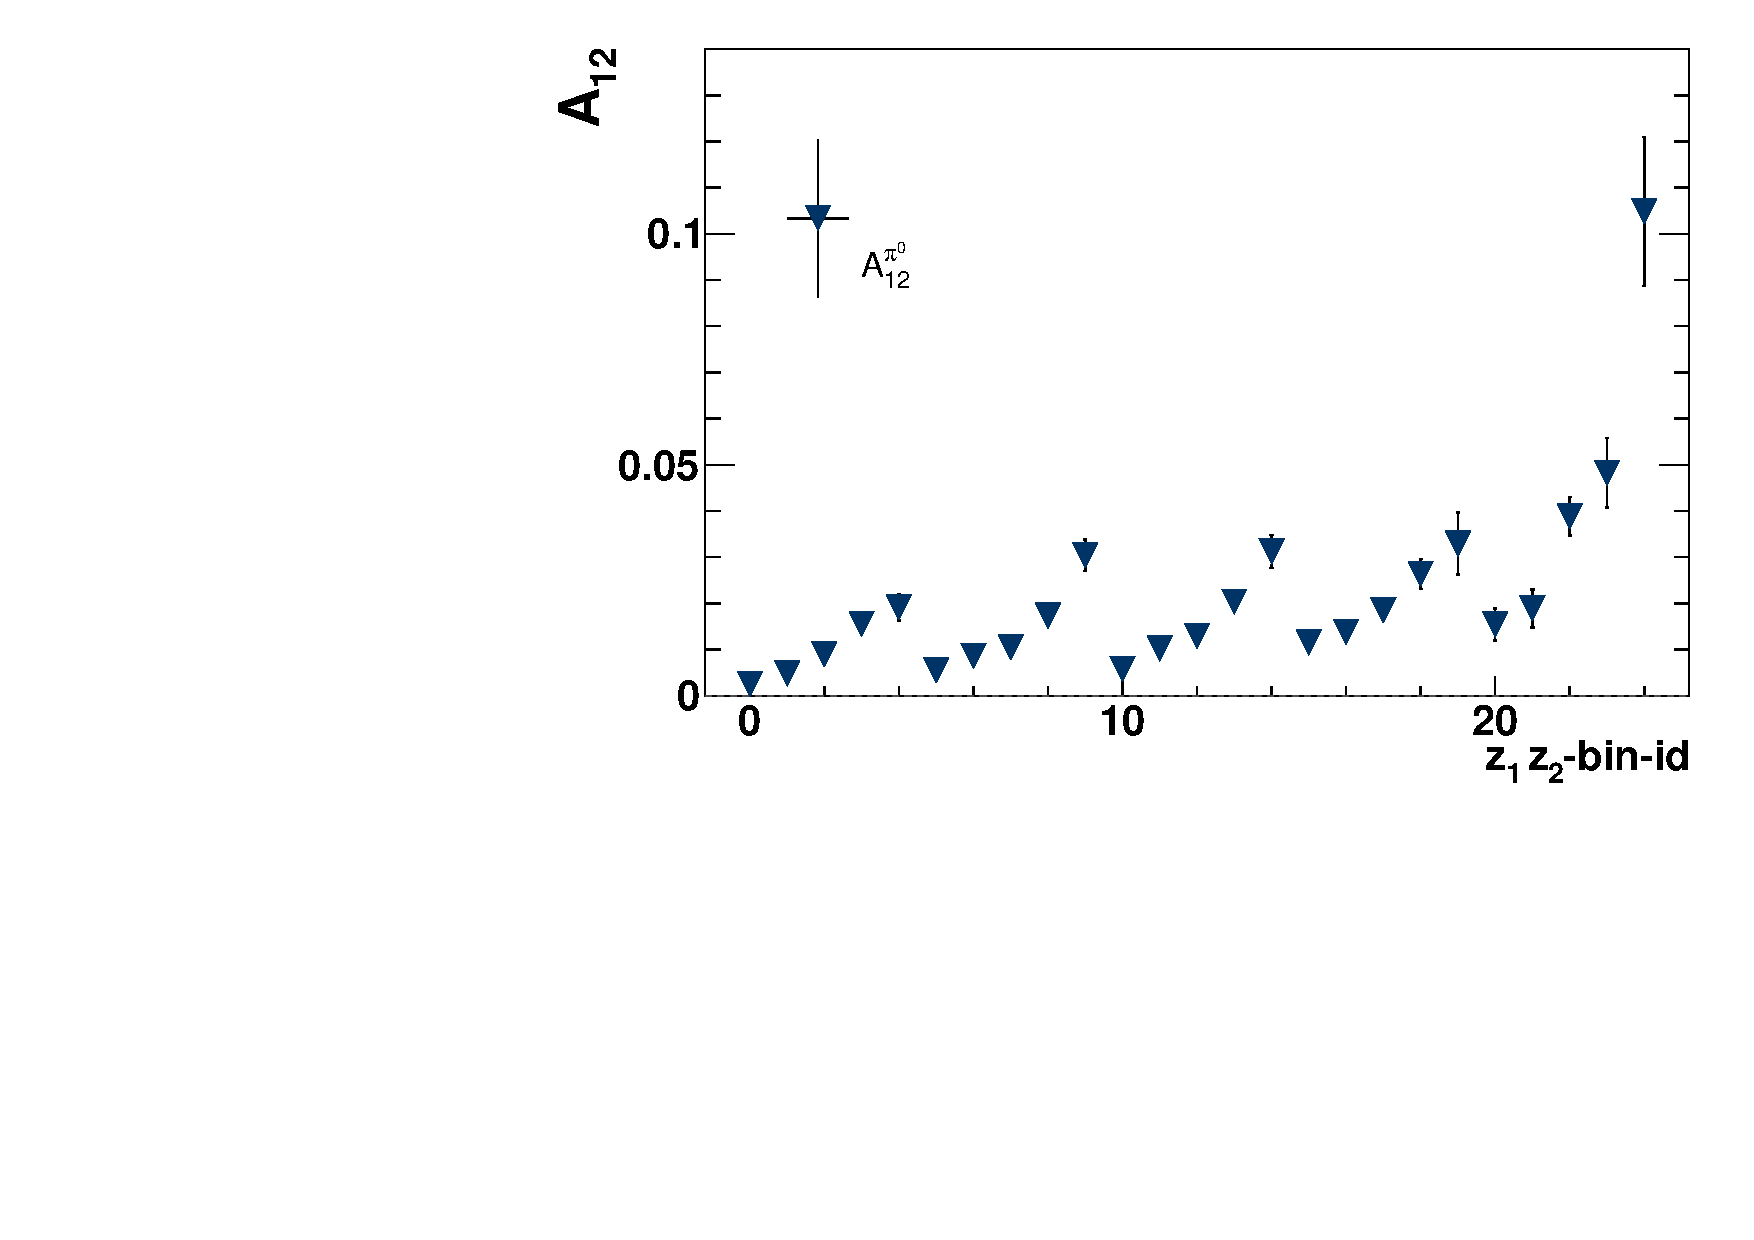
\includegraphics[width=.49\textwidth,natwidth=800,natheight=600]{figure_asy/Pi0NoCorrection1.pdf}}
  \subfigure[$\pi^0$ $(P_{t1},P_{t2})$ bins asymmetry]{\label{fig:exp_singlept1}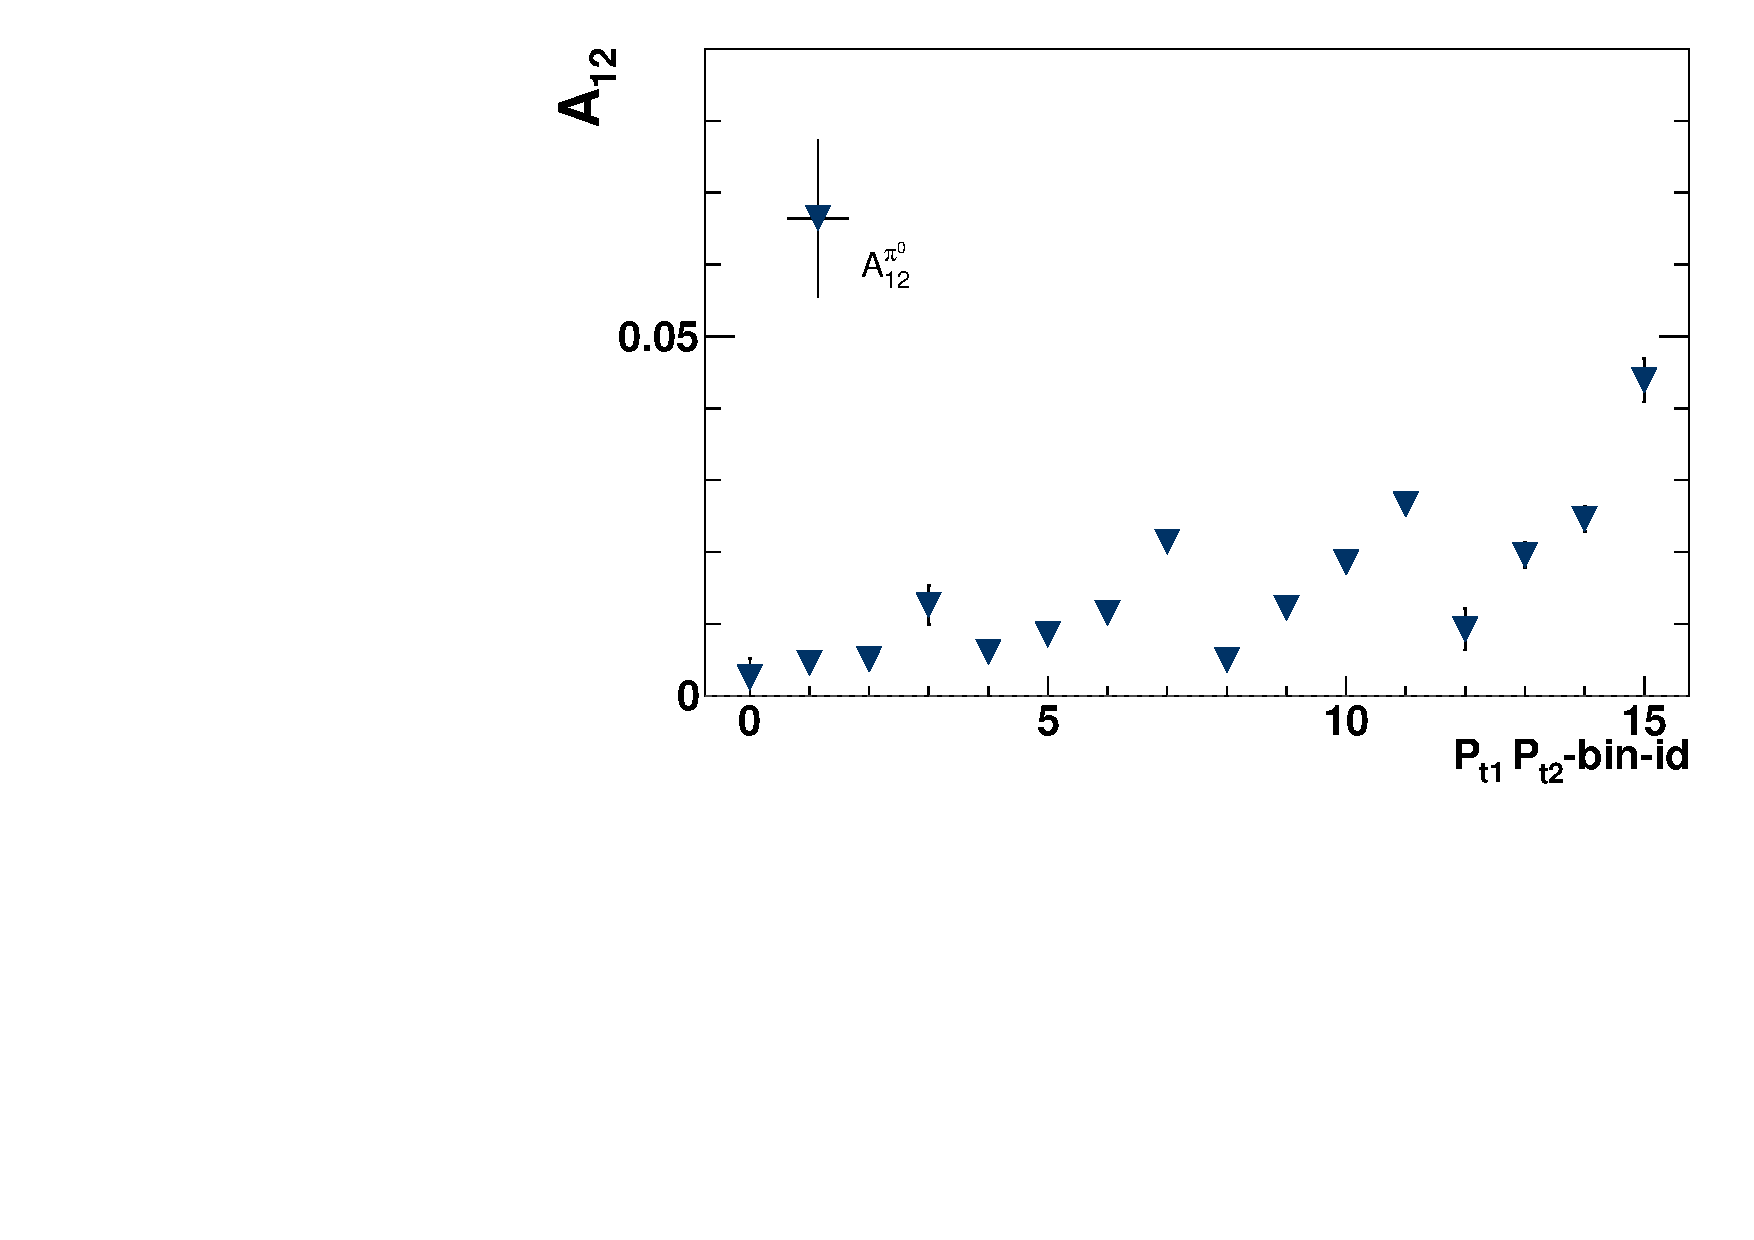
\includegraphics[width=.49\textwidth,natwidth=800,natheight=600]{figure_asy/Pi0NoCorrection3.pdf}}
  \caption{Experimental $\pi^0$ double-ratio Collins asymmetry $\nicefrac{A^{0\pm}_{12}}{A^L_{12}}$}
  \label{fig:exp_pi0_result}
\end{figure}

The result for the 2d binning in \(z_{i}\) (\(P_{ti}\)) has a more complicated pattern. It can be easily understood recalling the bin-numbering scheme shown in Figs.~\ref{fig:z1z2binning} and~\ref{fig:pt1pt2binning}. The extracted data points come in groups of five (four) points for which the kinematics of the second hadron is kept fixed and $z_1$ ($P_{t1}$) of the first hadron increases. Within these groups we observe a rise with $z_1$ ($P_{t1}$) and the average asymmetry in each group rises with $z_2$ and $P_{t2}$, as expected.


In Fig.~\ref{fig:exp_eta_result} we show the results for $A_{12}^{\eta}$ fitted to the $R_{12}^{\eta \pm}/R_{12}^L$ double ratio. Due to the higher mass of the $\eta$, we use the constraint $z> 0.3$, which is applied to all hadrons in double ratios containing $\eta$ mesons. Again, we observe significant asymmetries, rising both with \(z_i\) and \(P_{ti}\).  As the yields are lower, uncertainties are larger when compared to the corresponding $\pi^0$ asymmetries. 
\begin{figure}[H]
  \centering     
  \subfigure[$\eta$ $z_1$ bins asymmetry]{\label{fig:exp_singlez_eta}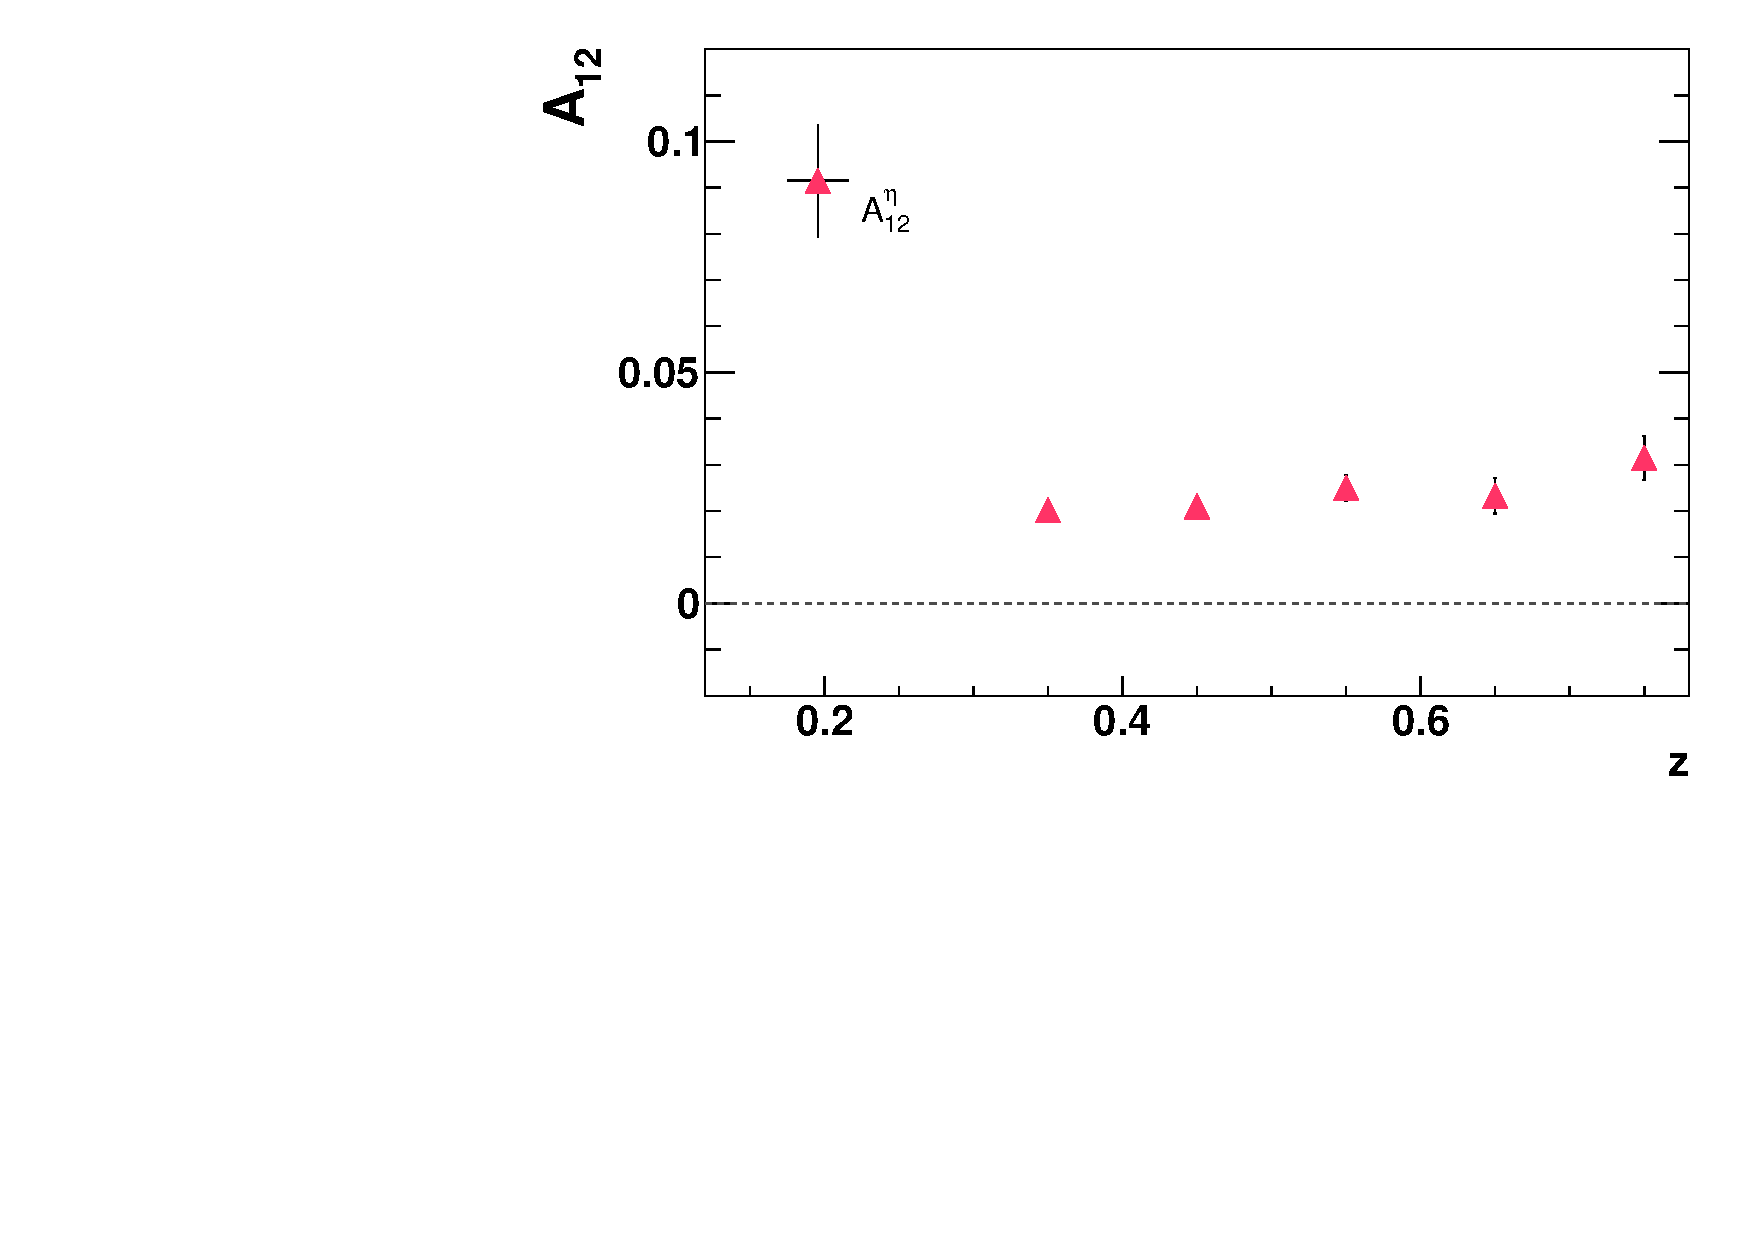
\includegraphics[width=.48\textwidth,natwidth=600,natheight=400]{figure_asy/EtaNoCorrection0.pdf}}
  \subfigure[$\eta$ $P_{t1}$ bins asymmetry]{\label{fig:exp_comz1_eta}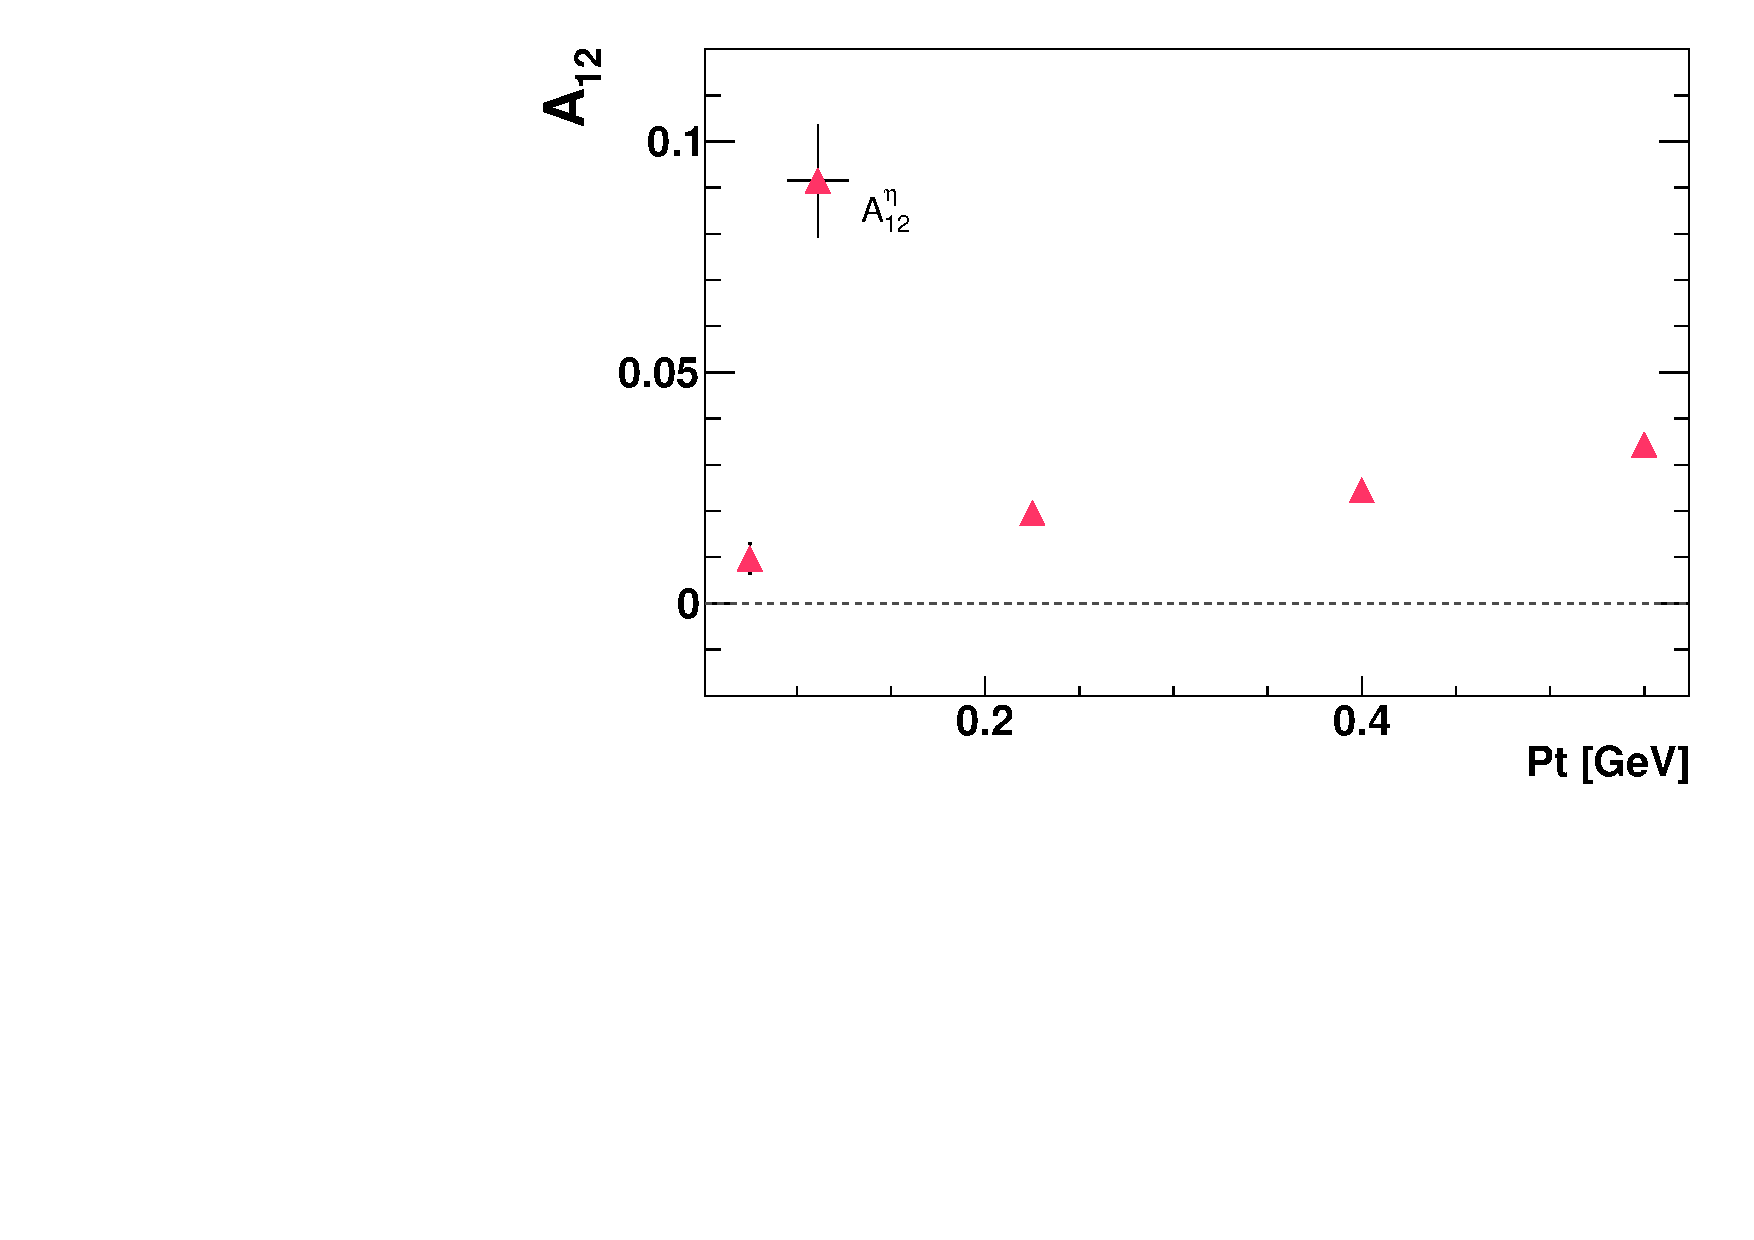
\includegraphics[width=.48\textwidth,natwidth=600,natheight=400]{figure_asy/EtaNoCorrection2.pdf}}
  \subfigure[$\eta$ $(z_1,z_2)$ bins asymmetry]{\label{fig:exp_singlept_eta}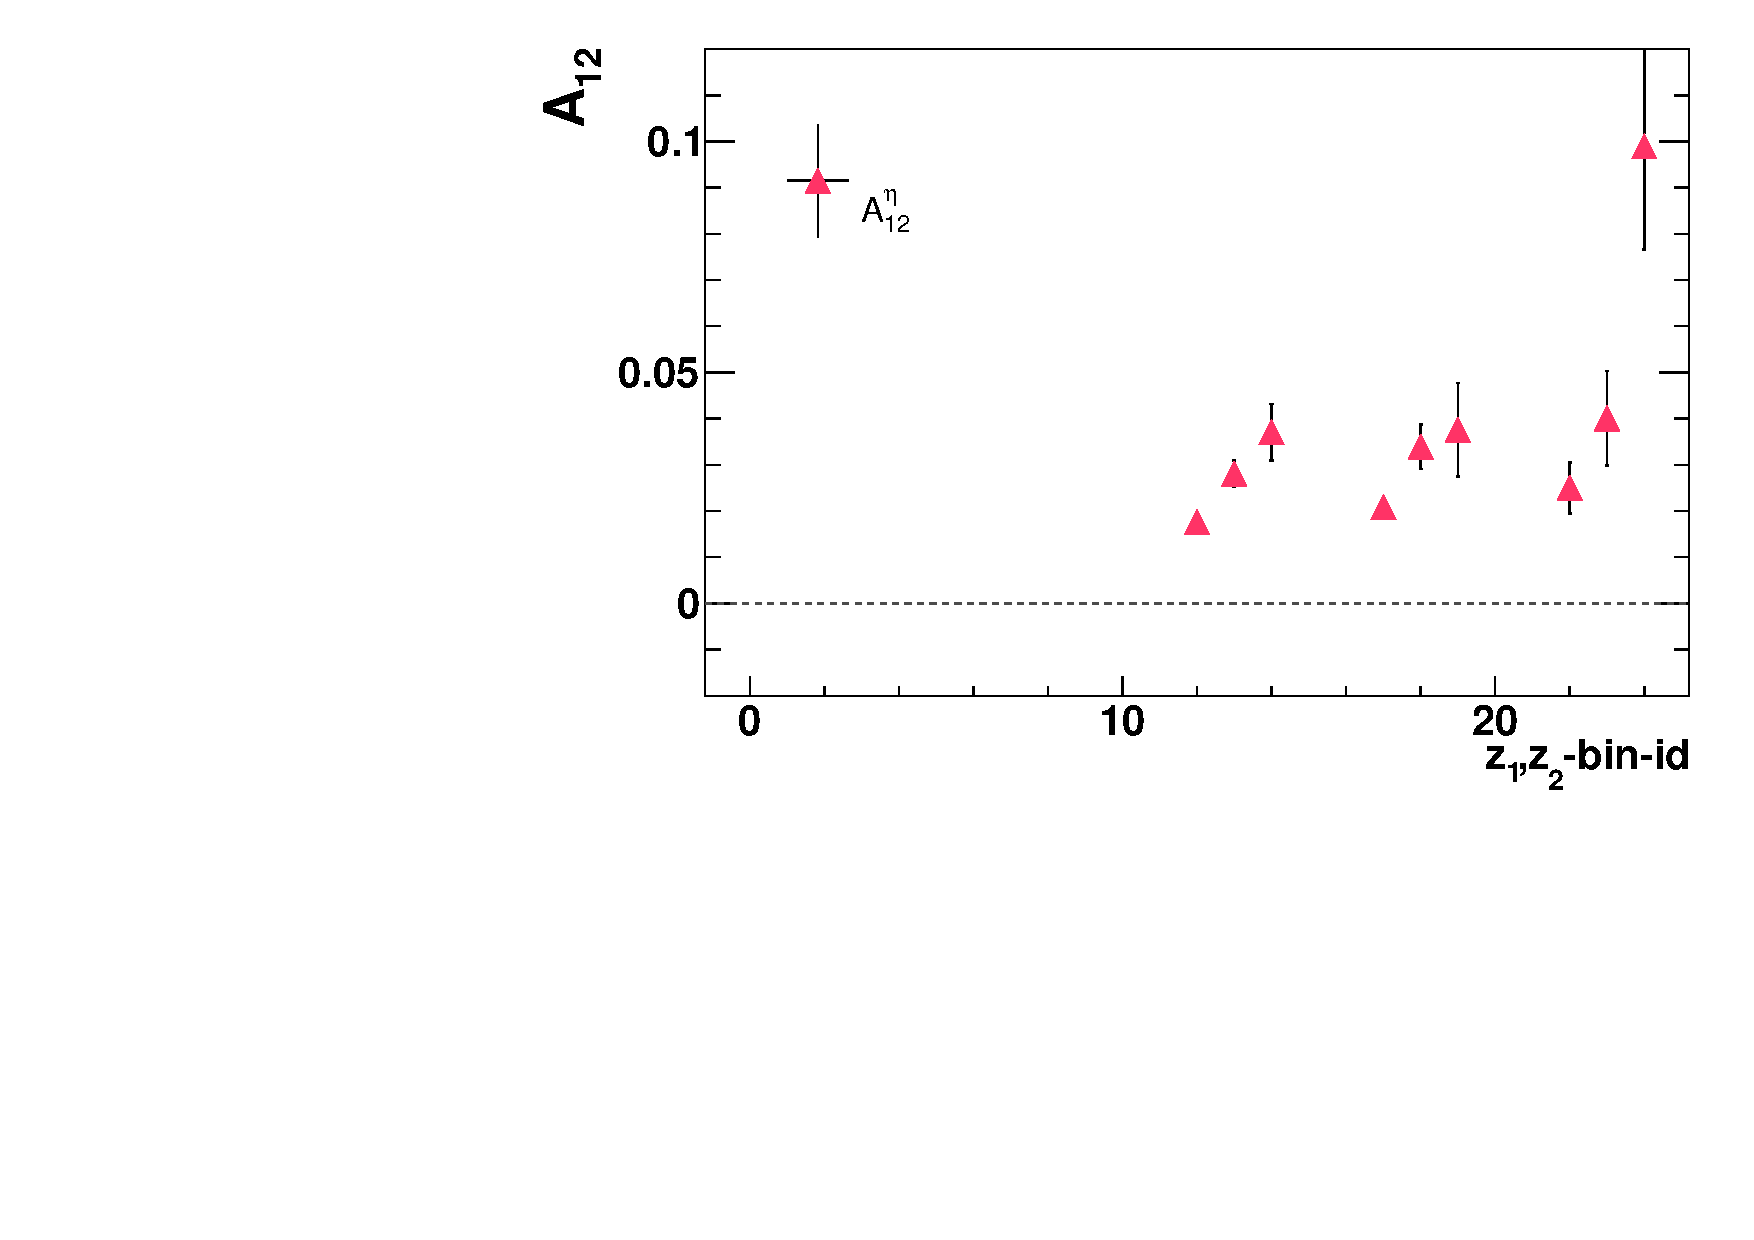
\includegraphics[width=.48\textwidth,natwidth=600,natheight=400]{figure_asy/EtaNoCorrection1.pdf}}
  \subfigure[$\eta$ $(P_{t1},P_{t2})$ bins asymmetry]{\label{fig:exp_compt1_eta}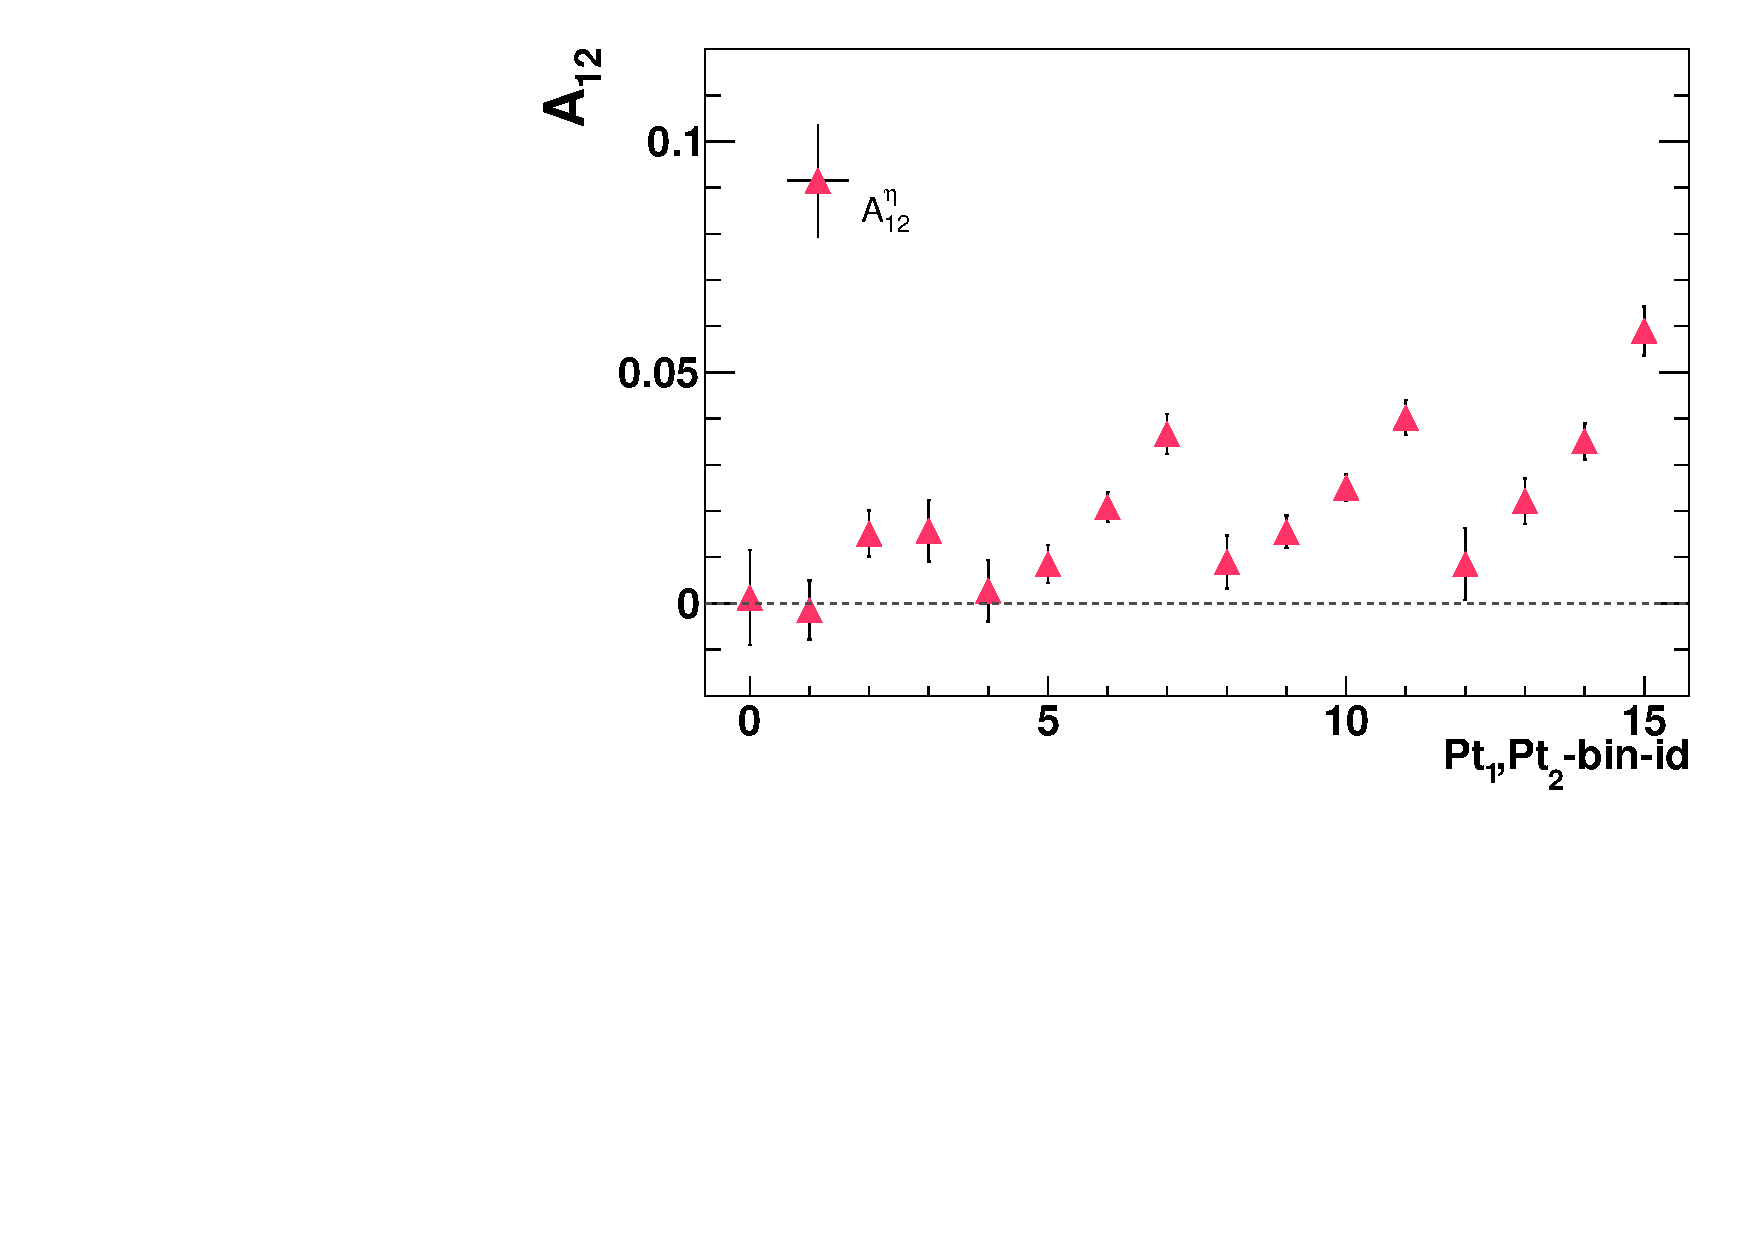
\includegraphics[width=.48\textwidth,natwidth=600,natheight=400]{figure_asy/EtaNoCorrection3.pdf}}
  \caption{Experimental $\eta$ double-ratio asymmetry $\nicefrac{A^{\eta\pm}_{12}}{A^L_{12}}$}
  \label{fig:exp_eta_result}
\end{figure}

%%%%%%%%%%%%%
\subsubsection{\texorpdfstring{Other Raw Asymmetries}{Other Raw Asymmetries}}

A difference of Collins asymmetries for $\eta$ and $\pi^0$ is of interest because it may explain the larger transverse single-spin asymmetry of $\eta$ observed in $pp$ collisions~\cite{StarTSSA2}. The $\eta$ has strangeness, which may cause such difference.
 
To compare asymmetries for $\eta$ and $\pi^0$, a threshold of $0.3$ for $z$ is applied to all hadrons, also for the $\pi^0$ double ratios. Figure~\ref{fig:exp_pi0_eta_result} displays  the comparison of $\pi^0$ and $\eta$ for the fractional-energy constraint $z>0.3$. 

\begin{figure}[t]
  \centering     
  \subfigure[$\pi^0$ and $\eta$ $z_1$ bins asymmetry]{\label{fig:exp_singlez_compare}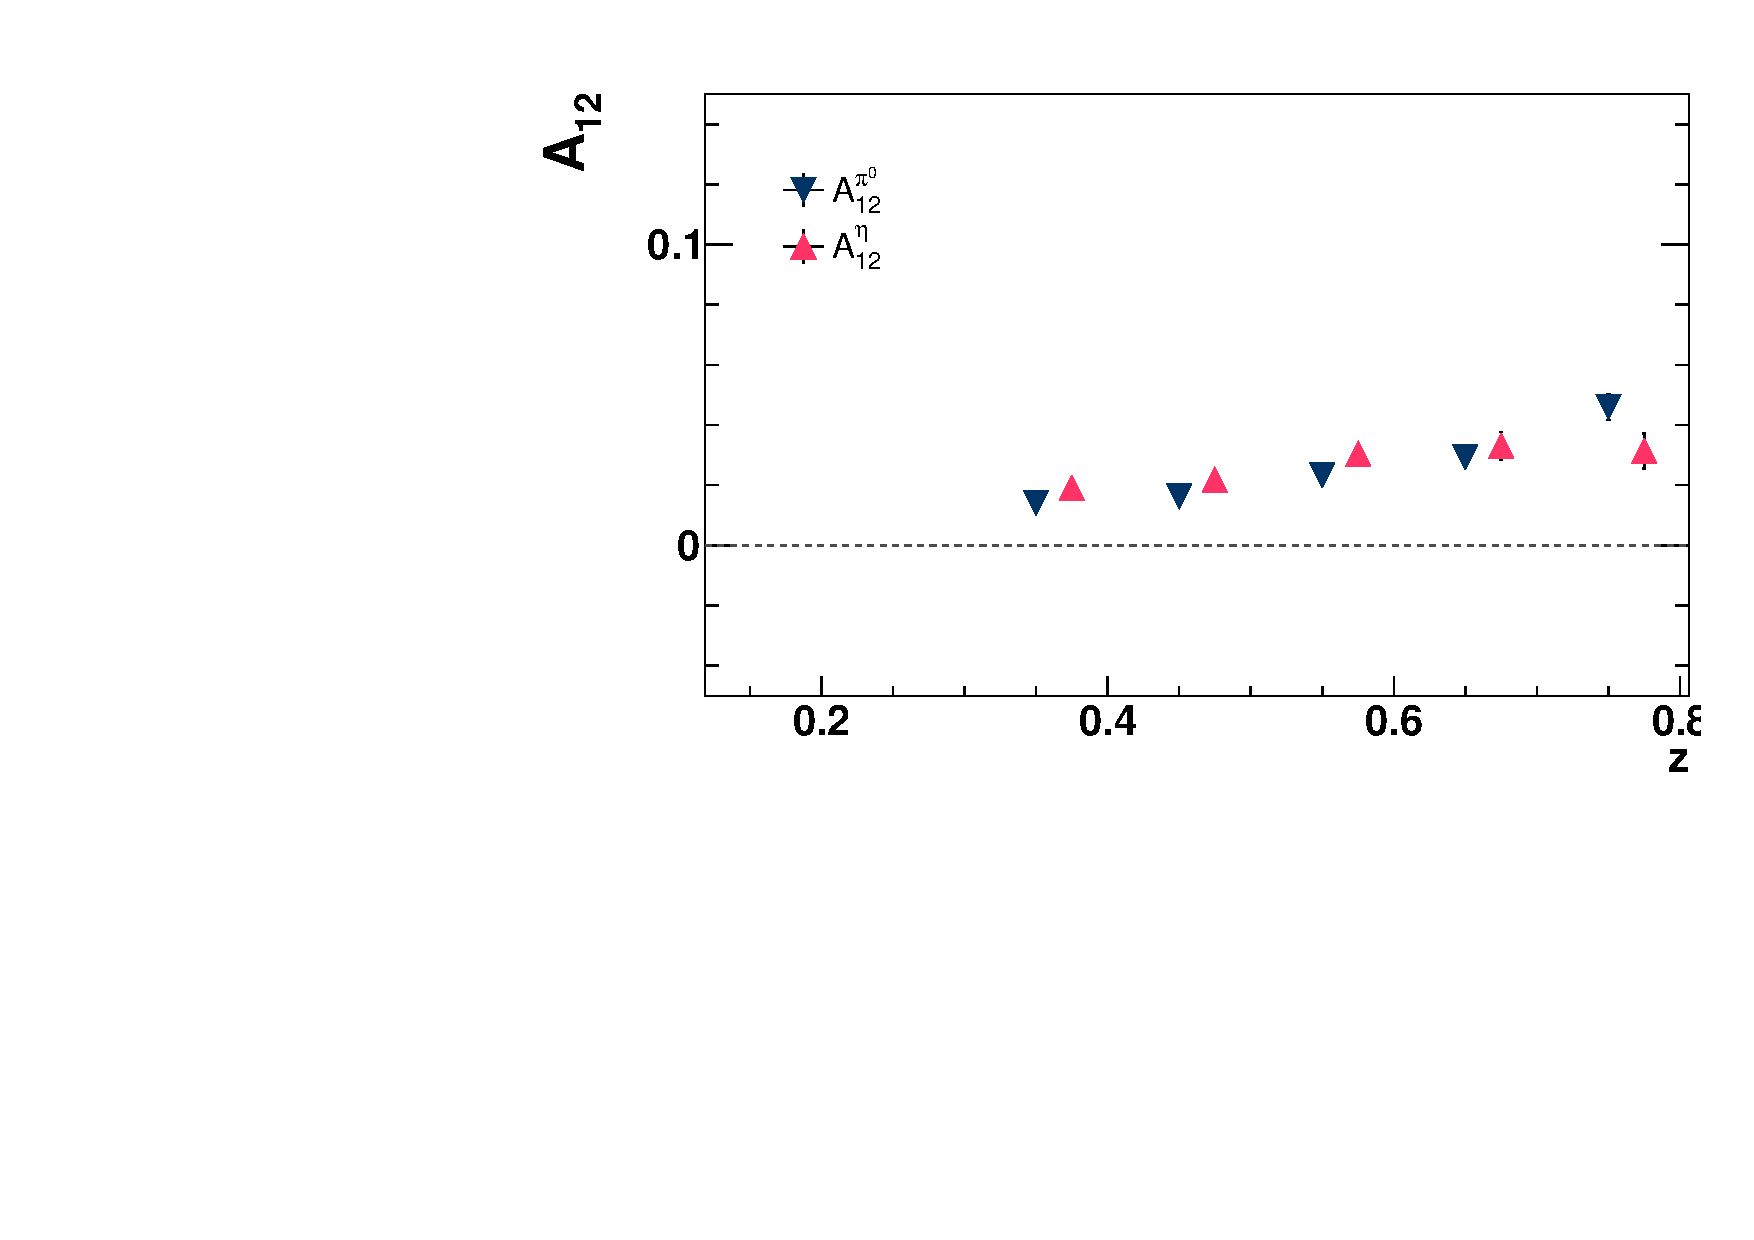
\includegraphics[width=.48\textwidth,natwidth=600,natheight=400]{figure_asy/Pi0VsEta0.pdf}}
  \subfigure[$\pi^0$ and $\eta$ $P_{t1}$ bins asymmetry]{\label{fig:exp_comz_compare}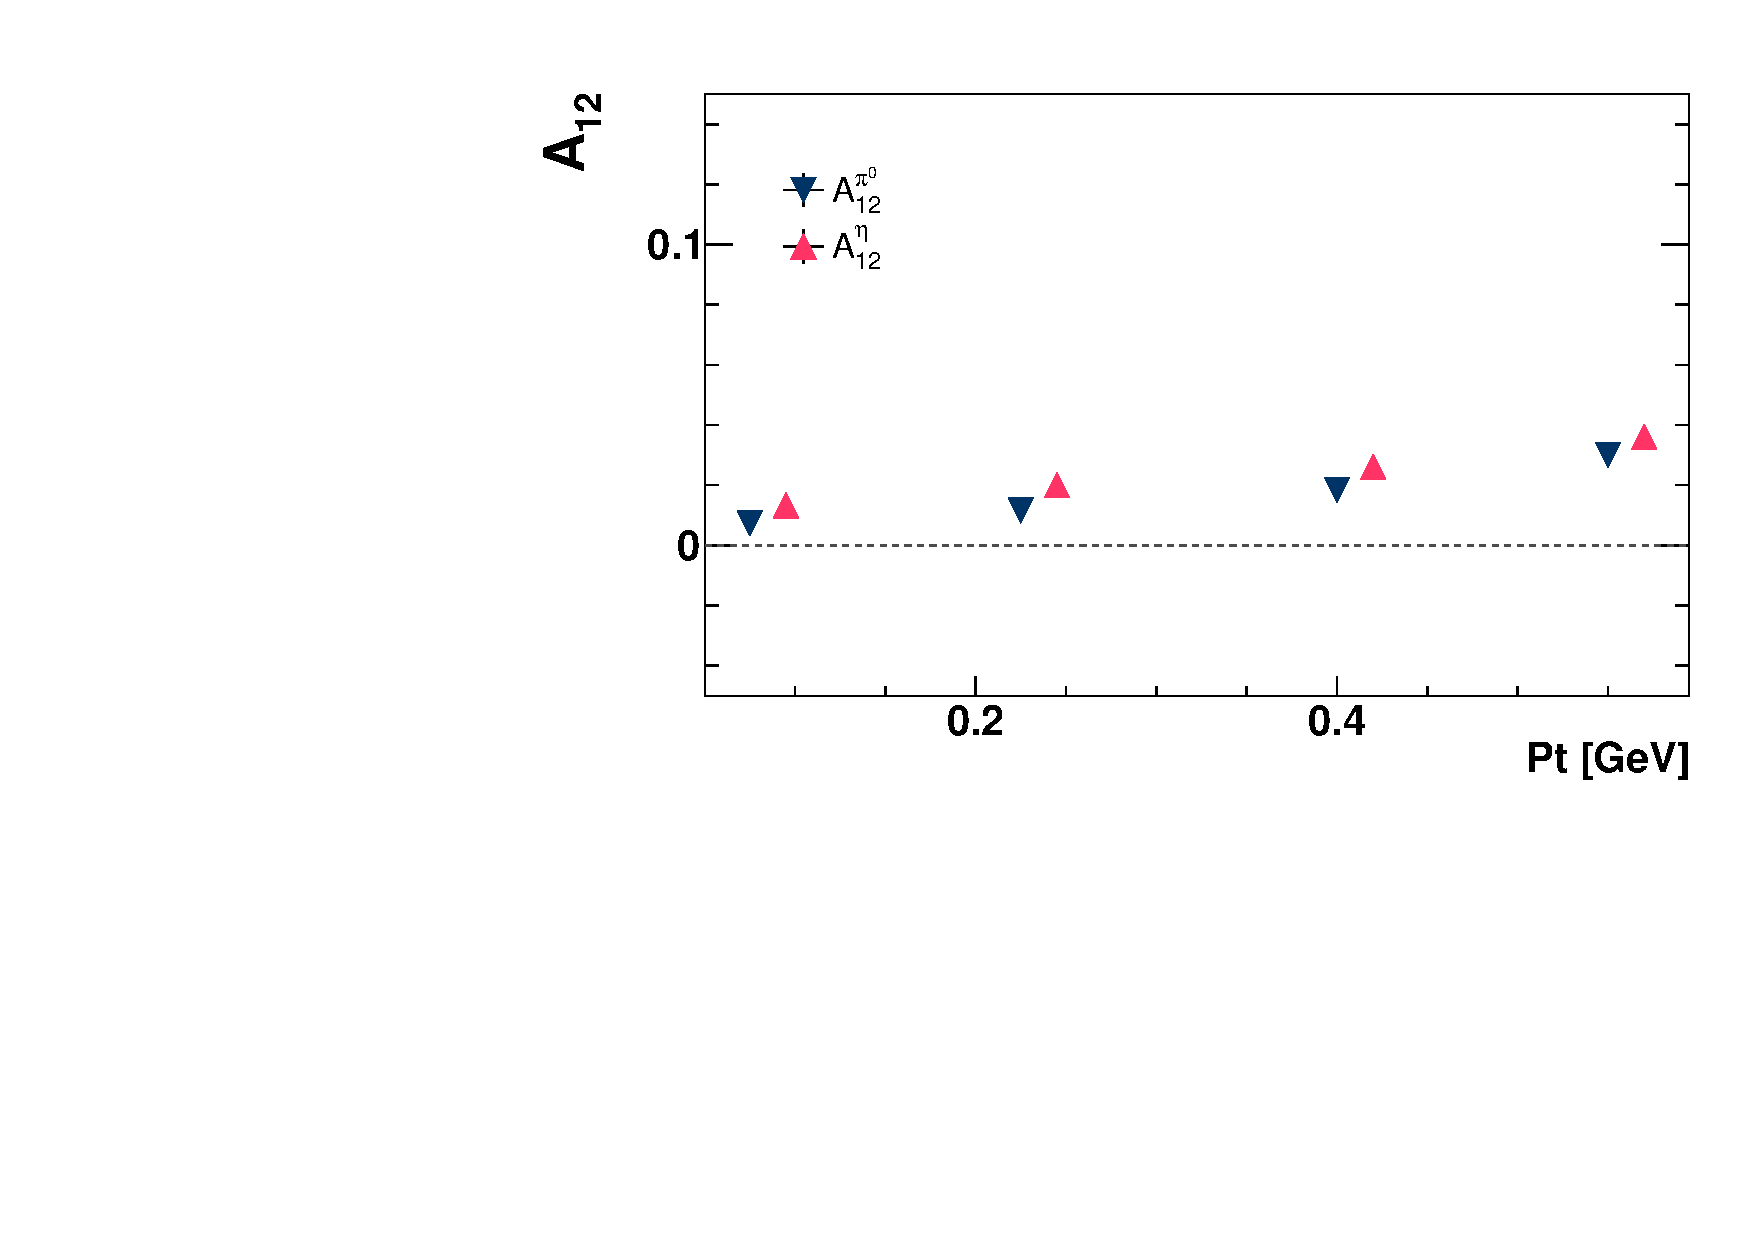
\includegraphics[width=.48\textwidth,natwidth=600,natheight=400]{figure_asy/Pi0VsEta2.pdf}}
  \subfigure[$\pi^0$ and $\eta$ $(z_1,z_2)$ bins asymmetry]{\label{fig:exp_singlept_compare}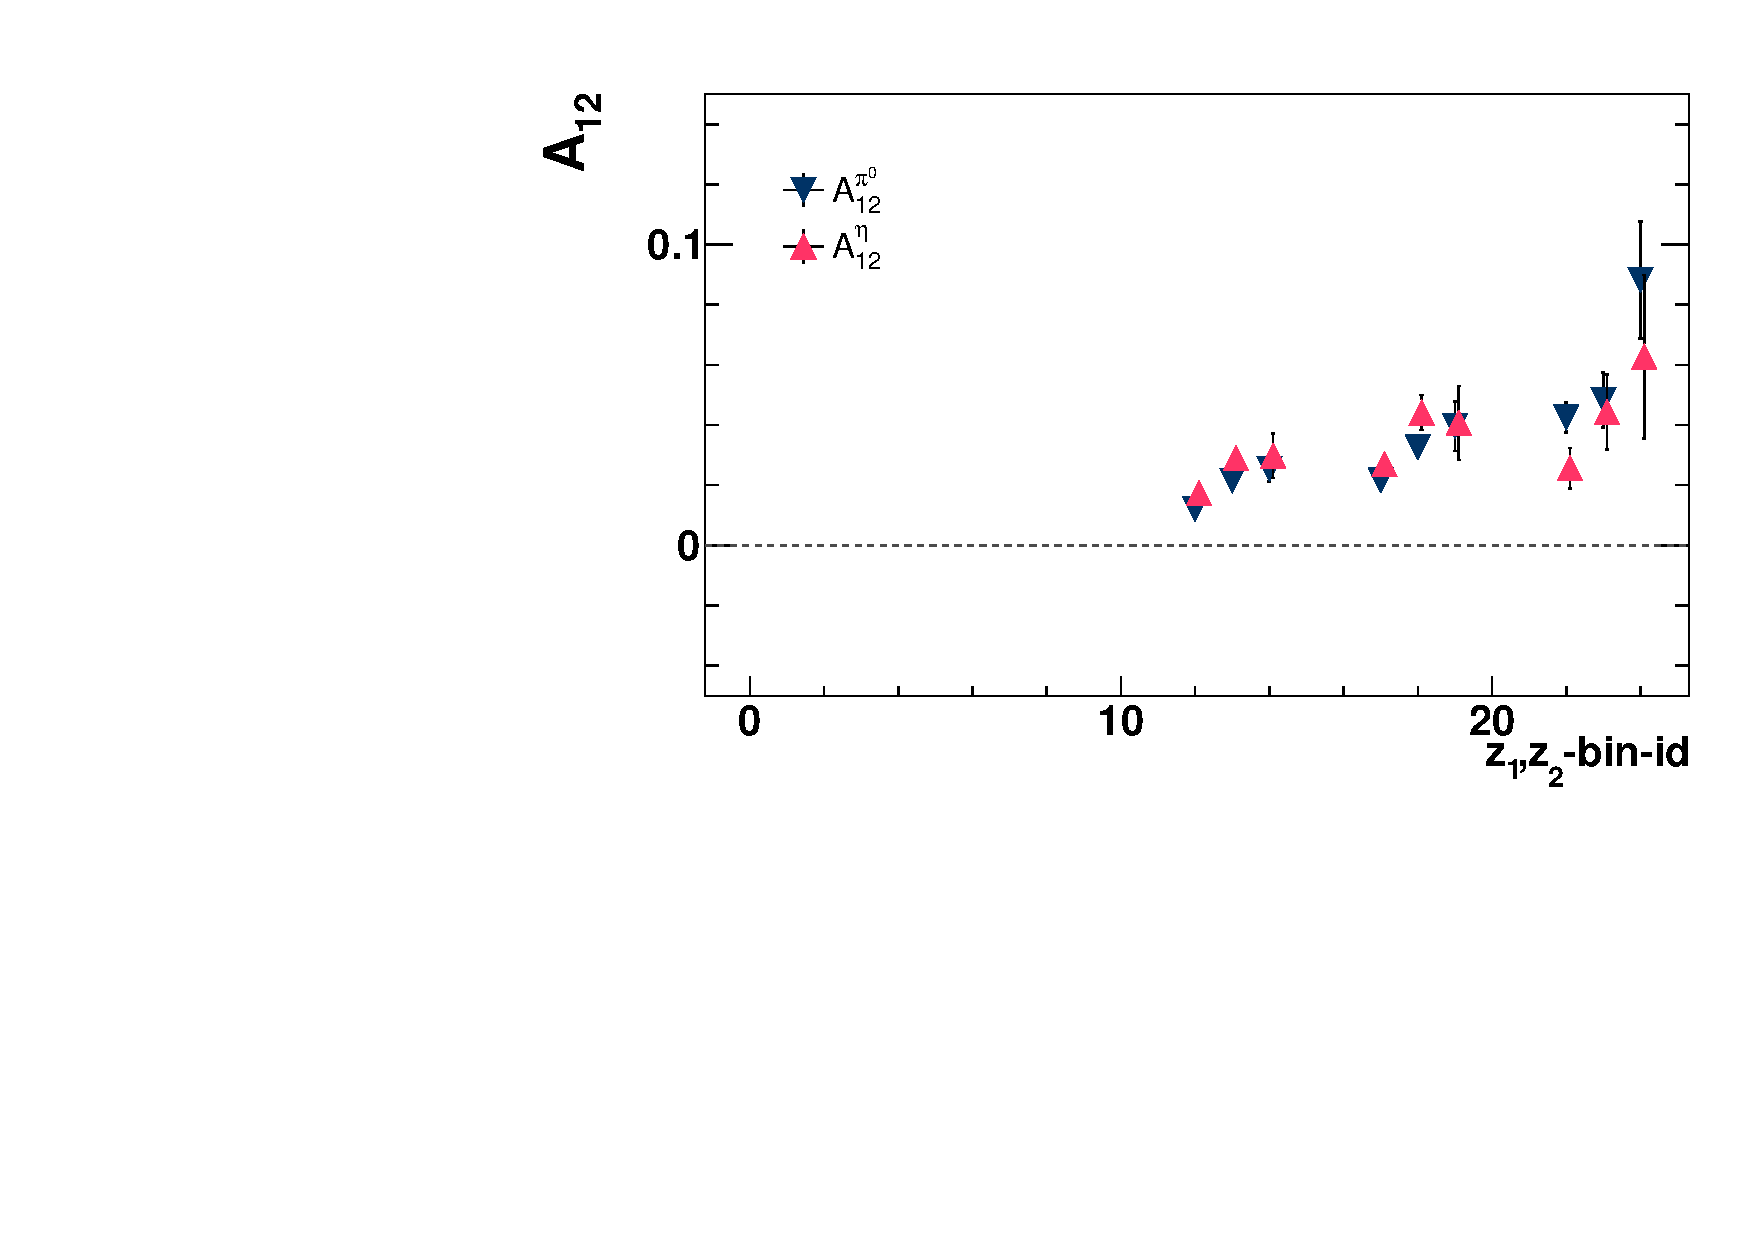
\includegraphics[width=.48\textwidth,natwidth=600,natheight=400]{figure_asy/Pi0VsEta1.pdf}}
  \subfigure[$\pi^0$ and $\eta$ $(P_{t1},P_{t2})$ bins asymmetry]{\label{fig:exp_compt_compare}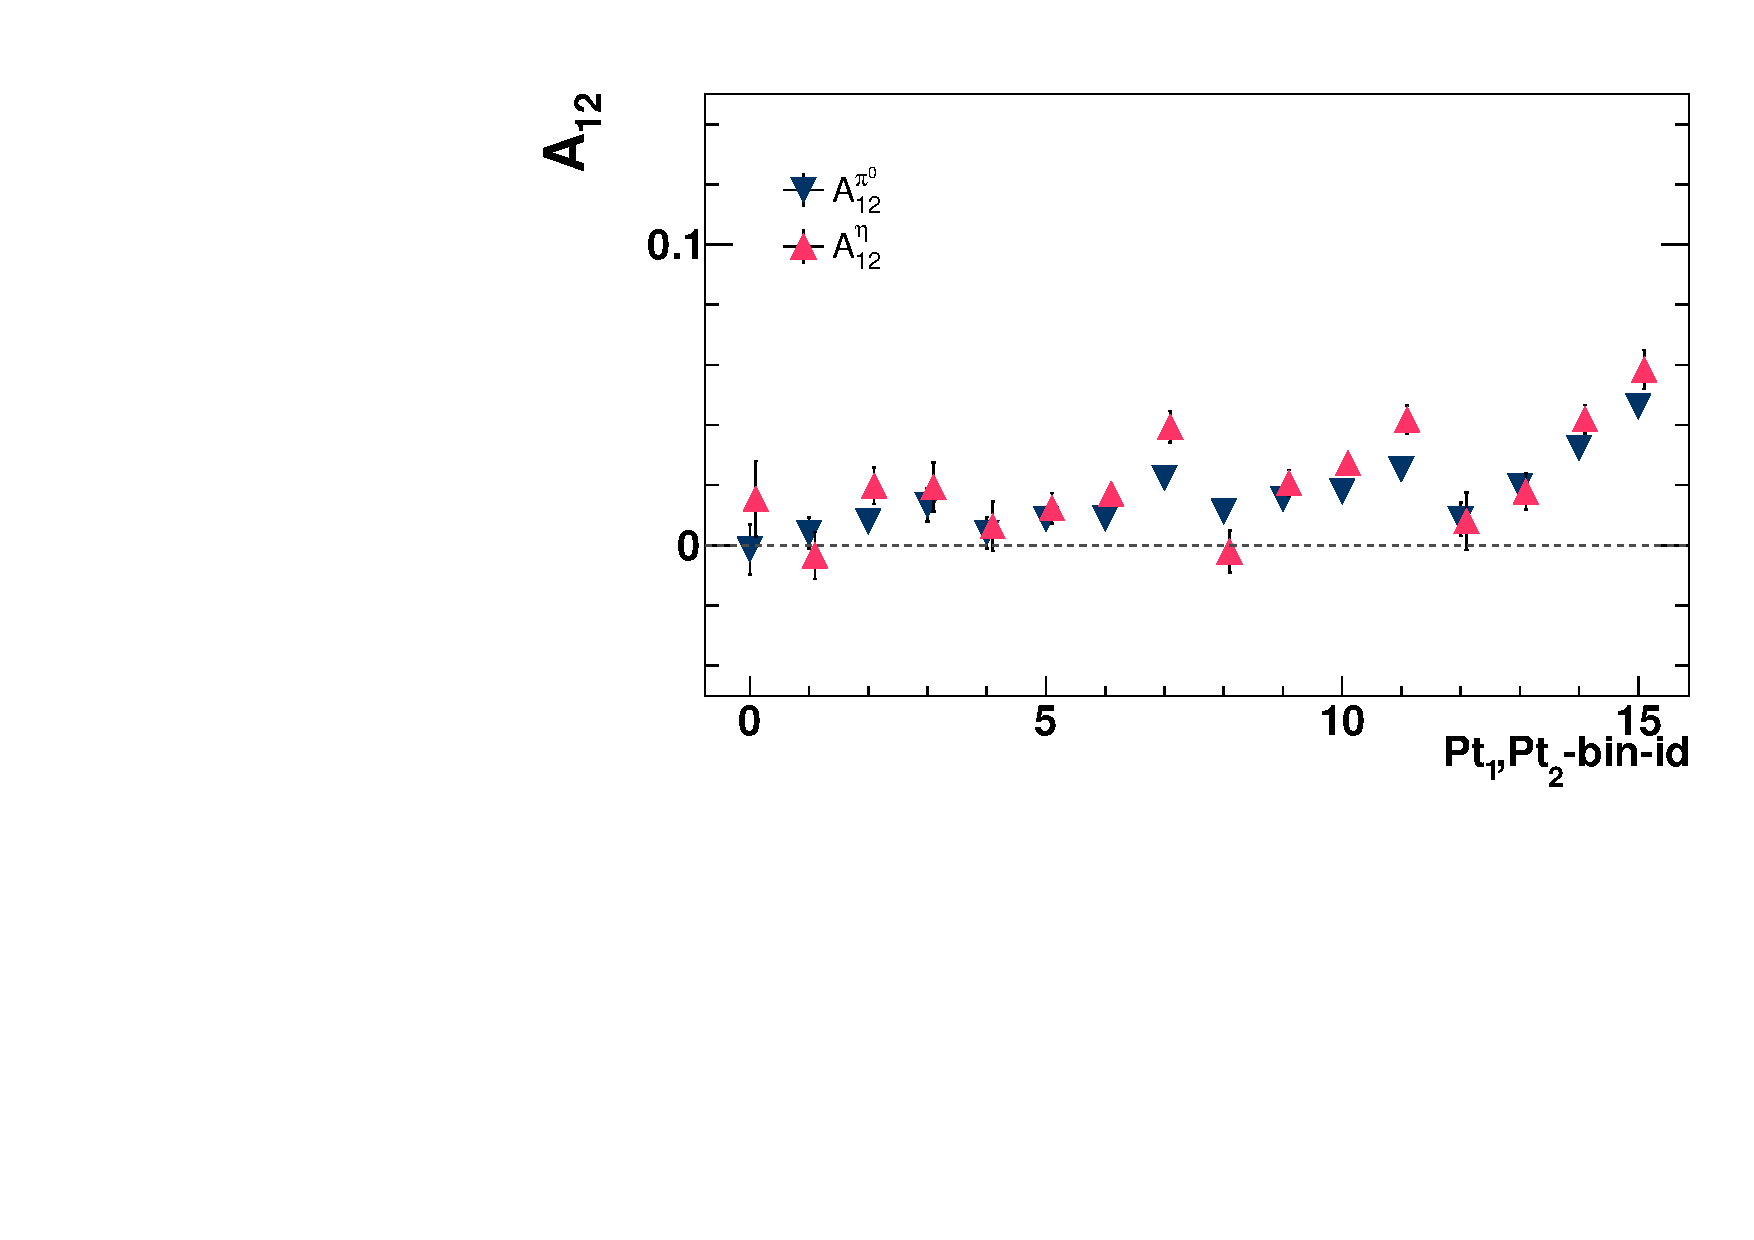
\includegraphics[width=.48\textwidth,natwidth=600,natheight=400]{figure_asy/Pi0VsEta3.pdf}}
  \caption[Comparison of $\pi^{0}$ and $\eta$ double-ratio asymmetries] {$\pi^0$ double ratio asymmetry $\nicefrac{A^{0\pm}_{12}}{A^L_{12}}$ and $\eta$ double ratio asymmetry $\nicefrac{A^{\eta\pm}_{12}}{A^L_{12}}$. The up pointing triangles are $\eta$ asymmetries and down pointing triangles are $\pi^0$ asymmetries.}
  \label{fig:exp_pi0_eta_result}
\end{figure}
Figure~\ref{fig:exp_pi0_eta_ratio} shows the asymmetries of the $\eta$--$\pi^0$ double ratio. Within the uncertainties the asymmetries are consistent with zero. However, at the highest $z$ and $P_t$ values there is a hint of an excess of $A_{12}^\eta$ over the asymmetries constructed with the neutral pion.
%Besides the uncertainty caused by statistics, $\pi^0$ shows different asymmetries than $\eta$ at some bins. This could be caused by, eg., the expected difference in the fragmentation of strange quarks or by differences between detection efficiencies of $\pi^0$ and $\eta$. However, this difference is nonsignificant at this stage and more precise conclusion will be discussed after the correction of thrust smearing effect.
\begin{figure}[H]
  \centering     
  \subfigure[$\pi^0$ over $\eta$ double ratio $z_1$ bins]{\label{fig:exp_singlez_ratio}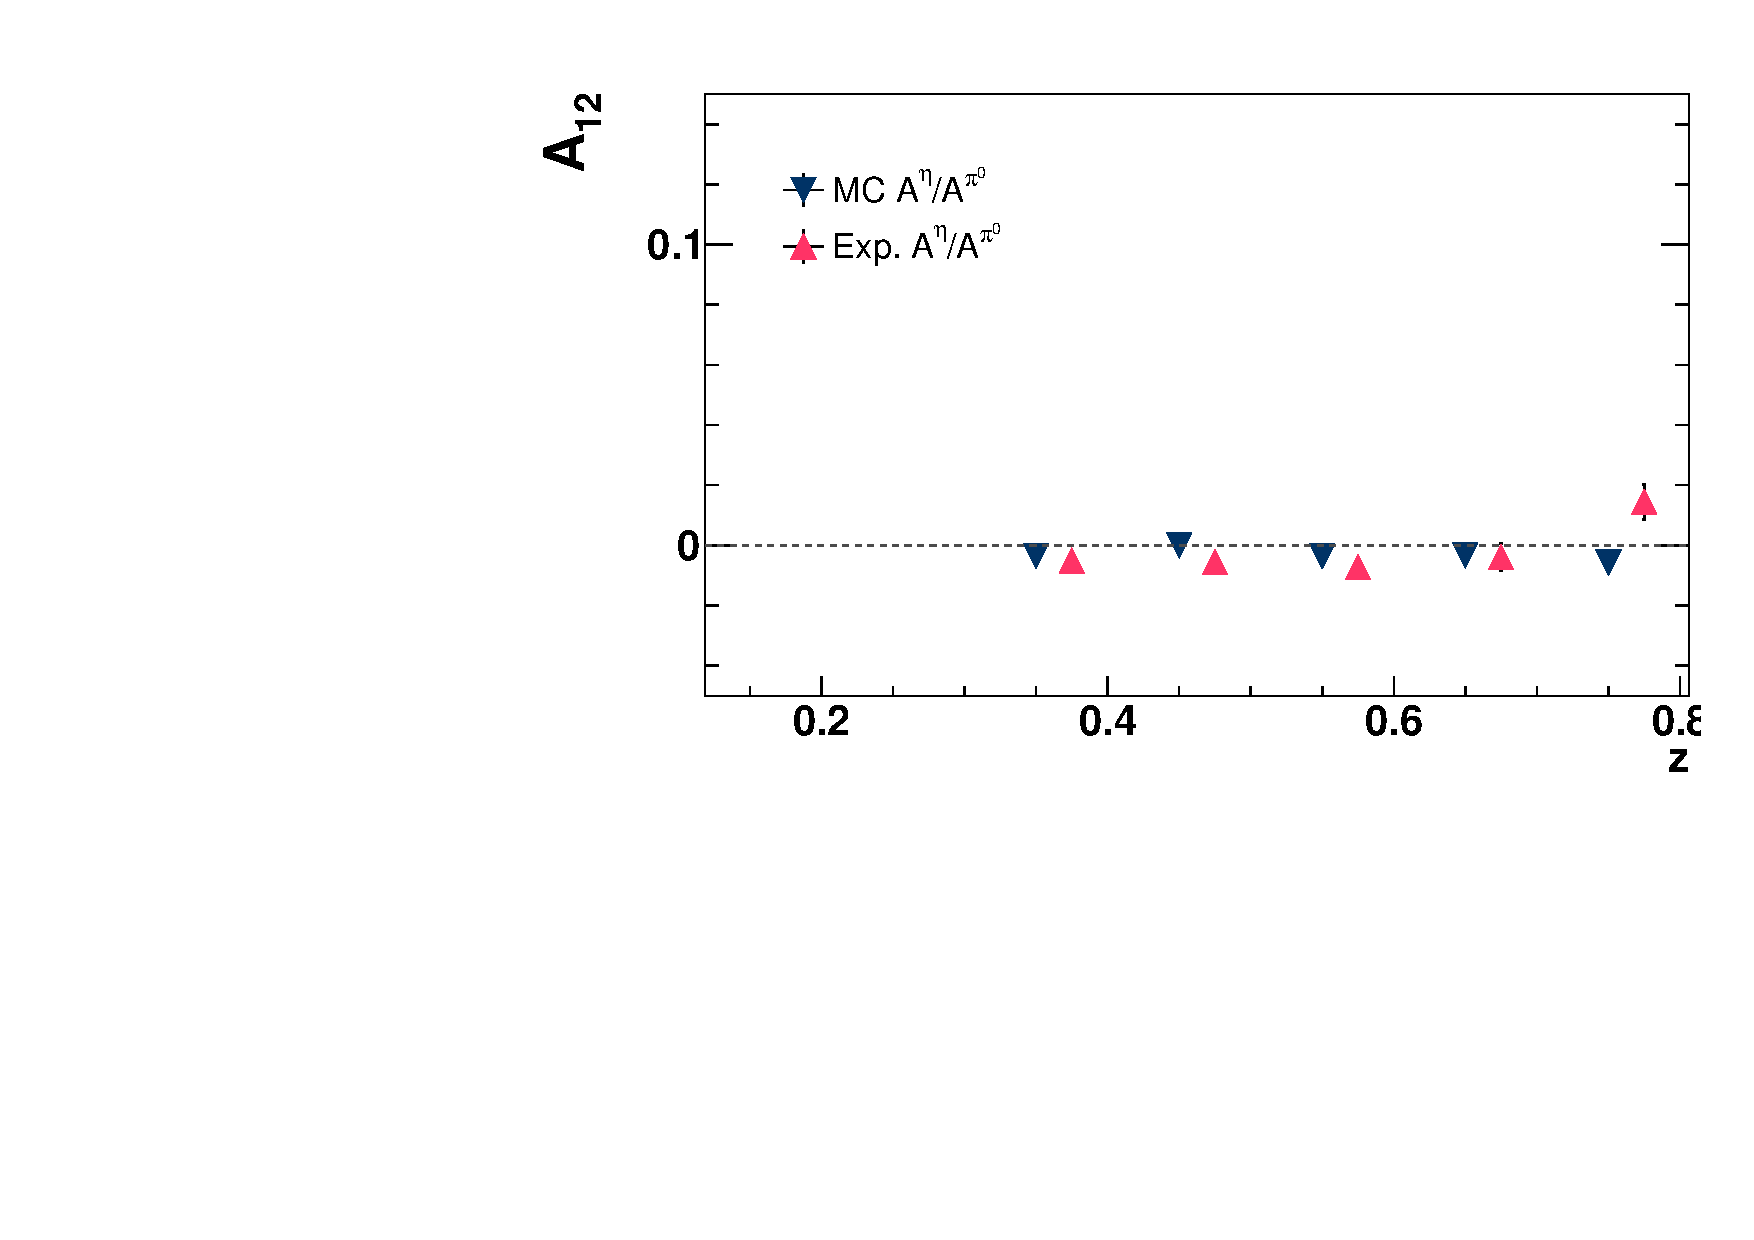
\includegraphics[width=.48\textwidth,natwidth=600,natheight=400]{figure_asy/Pi0OverEta0.pdf}}
   \subfigure[$\pi^0$ over $\eta$ double ratio $P_{t1}$ bins]{\label{fig:exp_comz_ratio}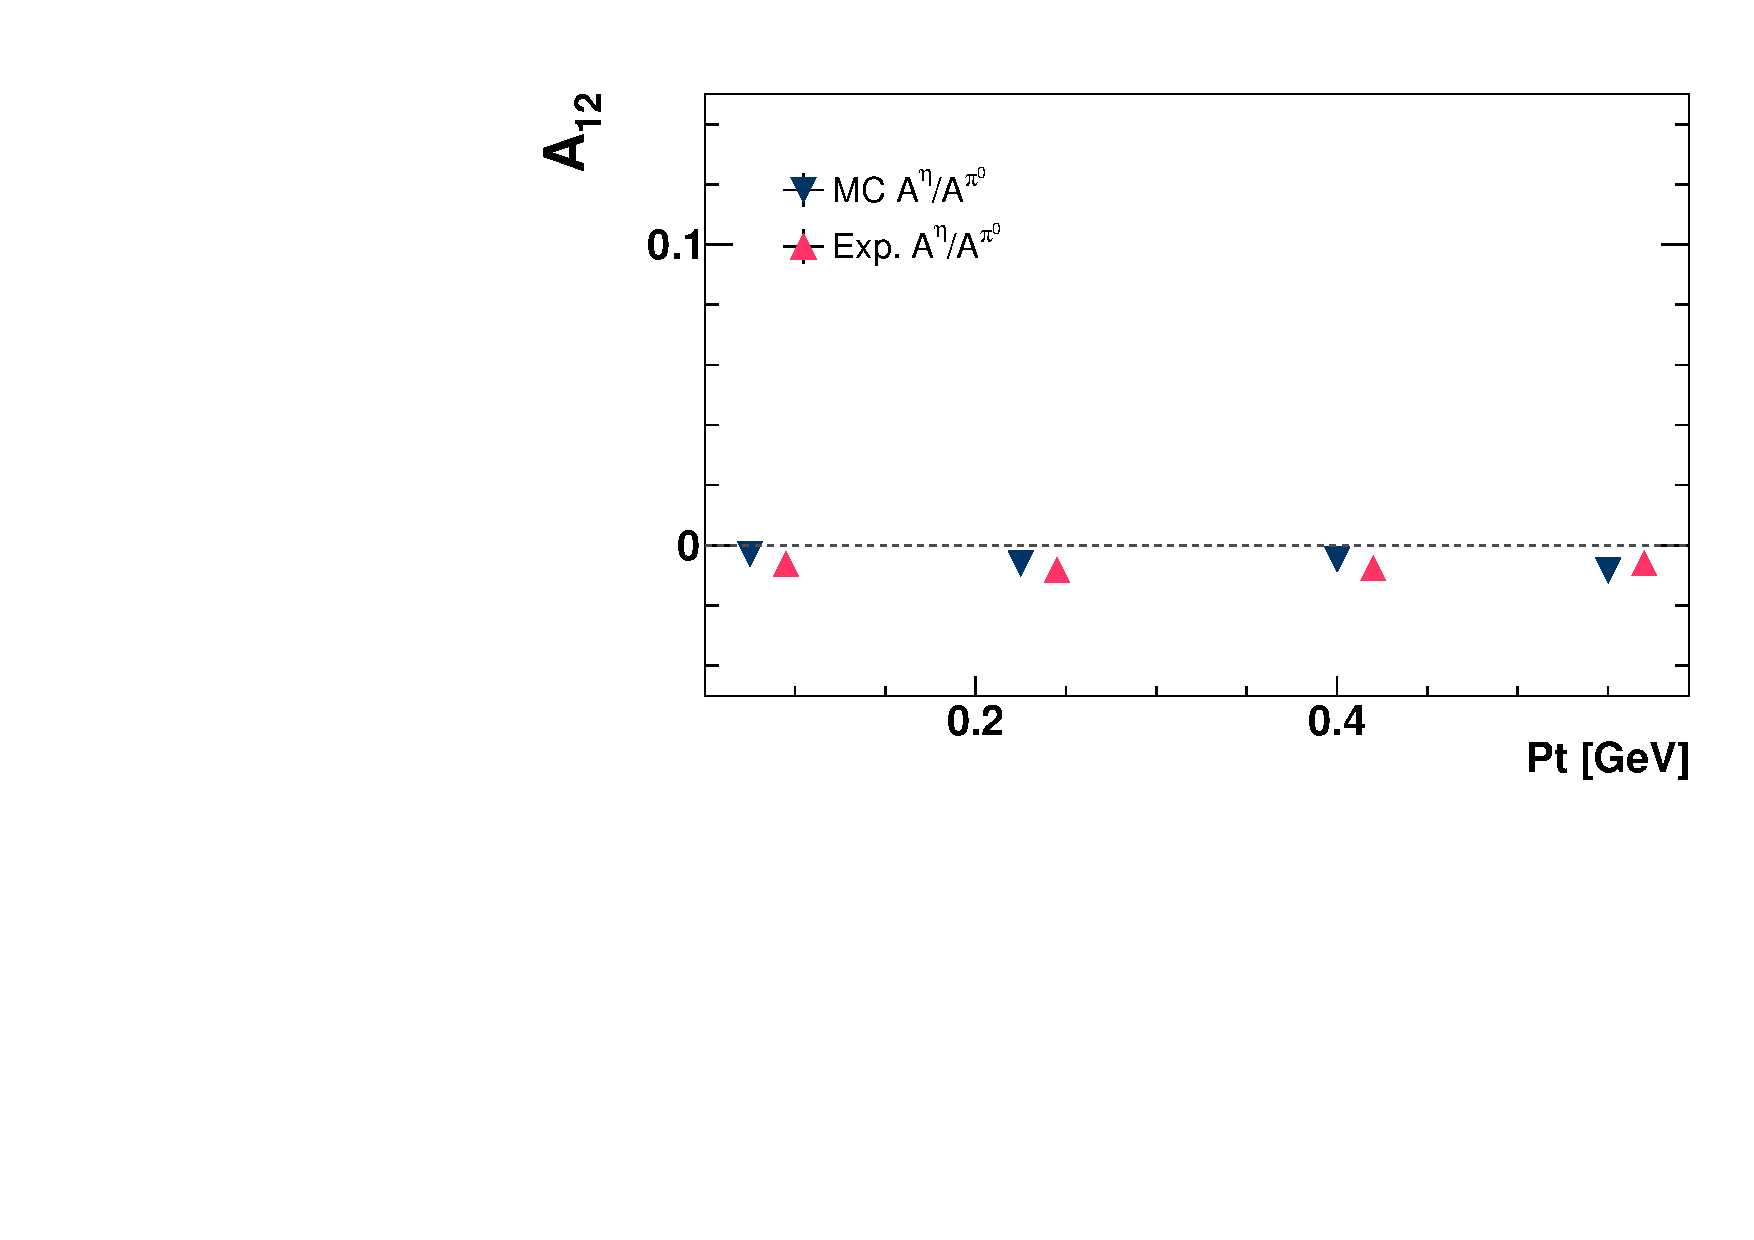
\includegraphics[width=.48\textwidth,natwidth=600,natheight=400]{figure_asy/Pi0OverEta2.pdf}}
  \subfigure[$\pi^0$ over $\eta$ double ratio $(z_1,z_2)$ bins]{\label{fig:exp_signlept_ratio}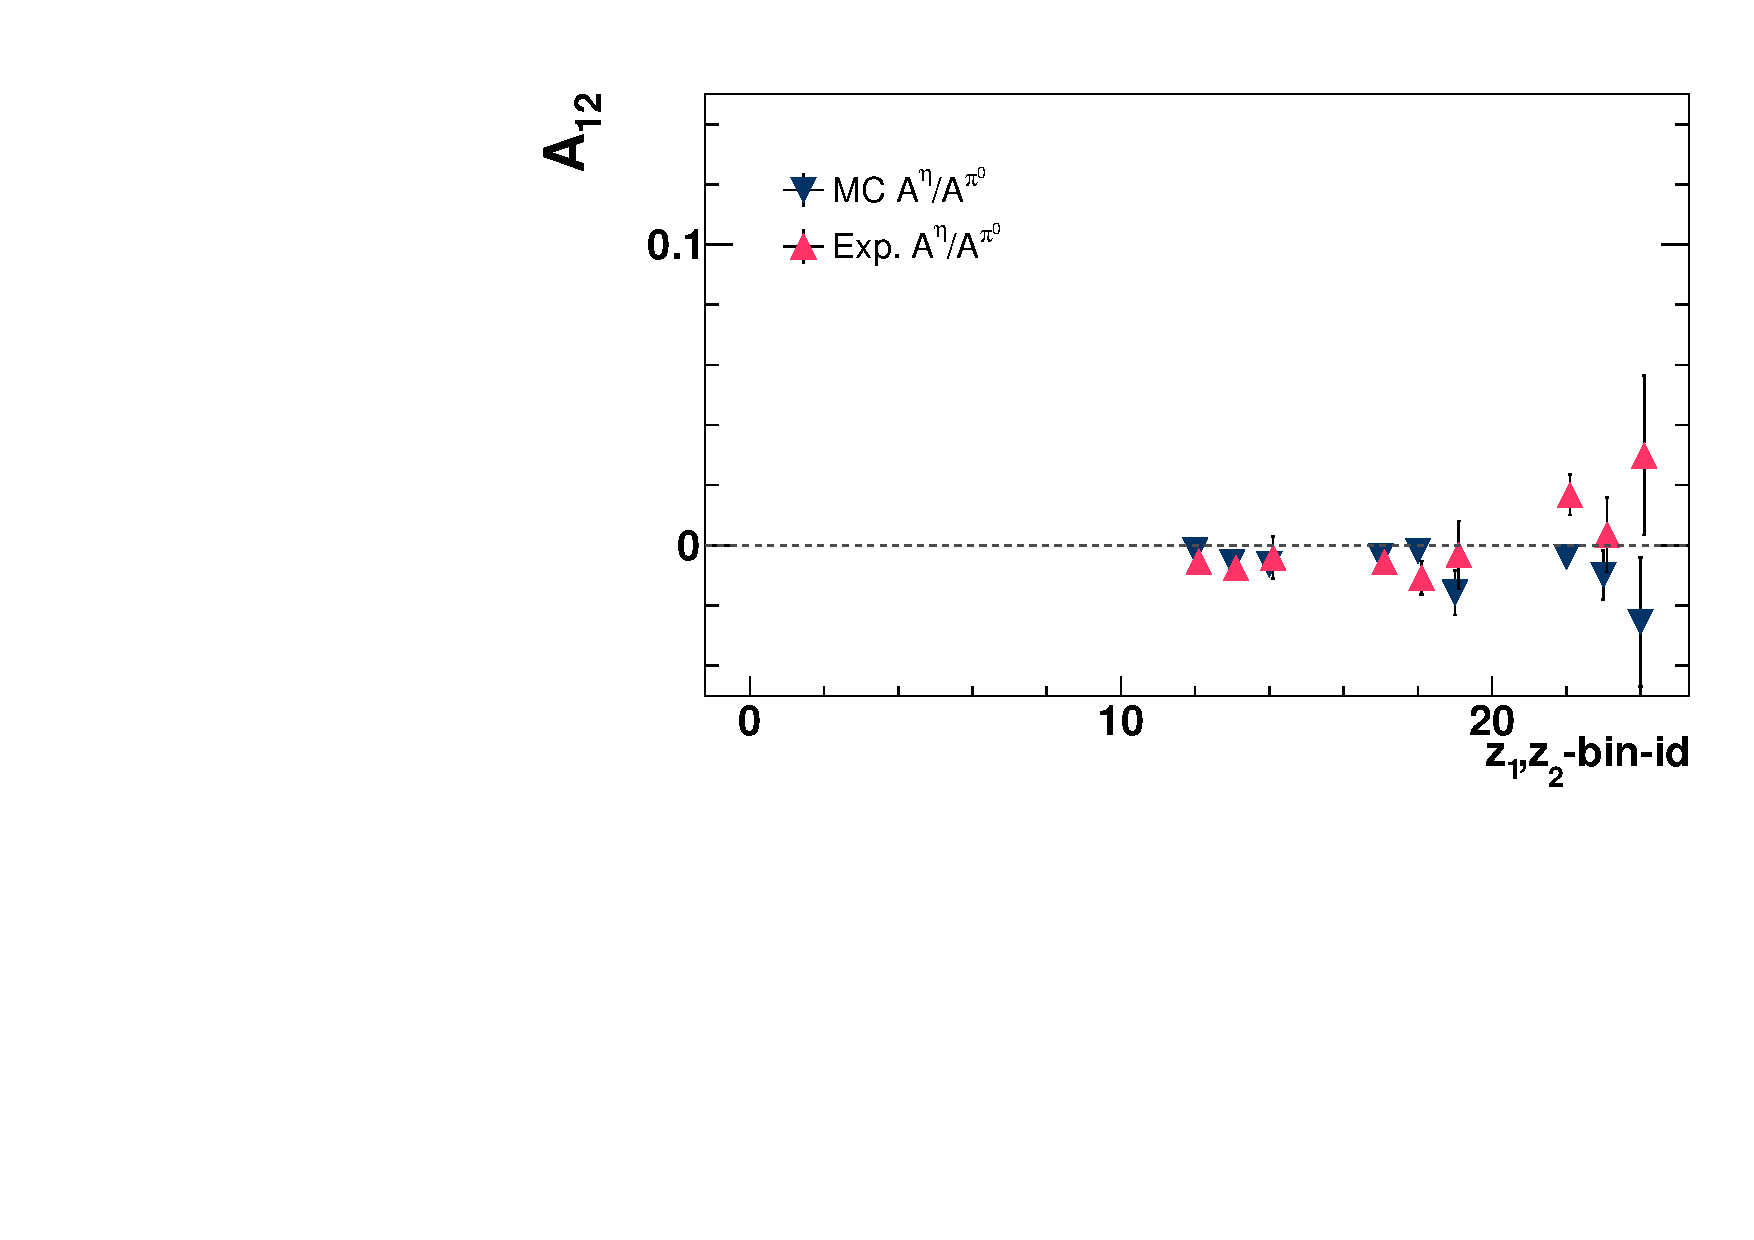
\includegraphics[width=.48\textwidth,natwidth=600,natheight=400]{figure_asy/Pi0OverEta1.pdf}}
  \subfigure[$\pi^0$ over $\eta$ double ratio $(P_{t1},P_{t2})$ bins]{\label{fig:exp_compt_ratio}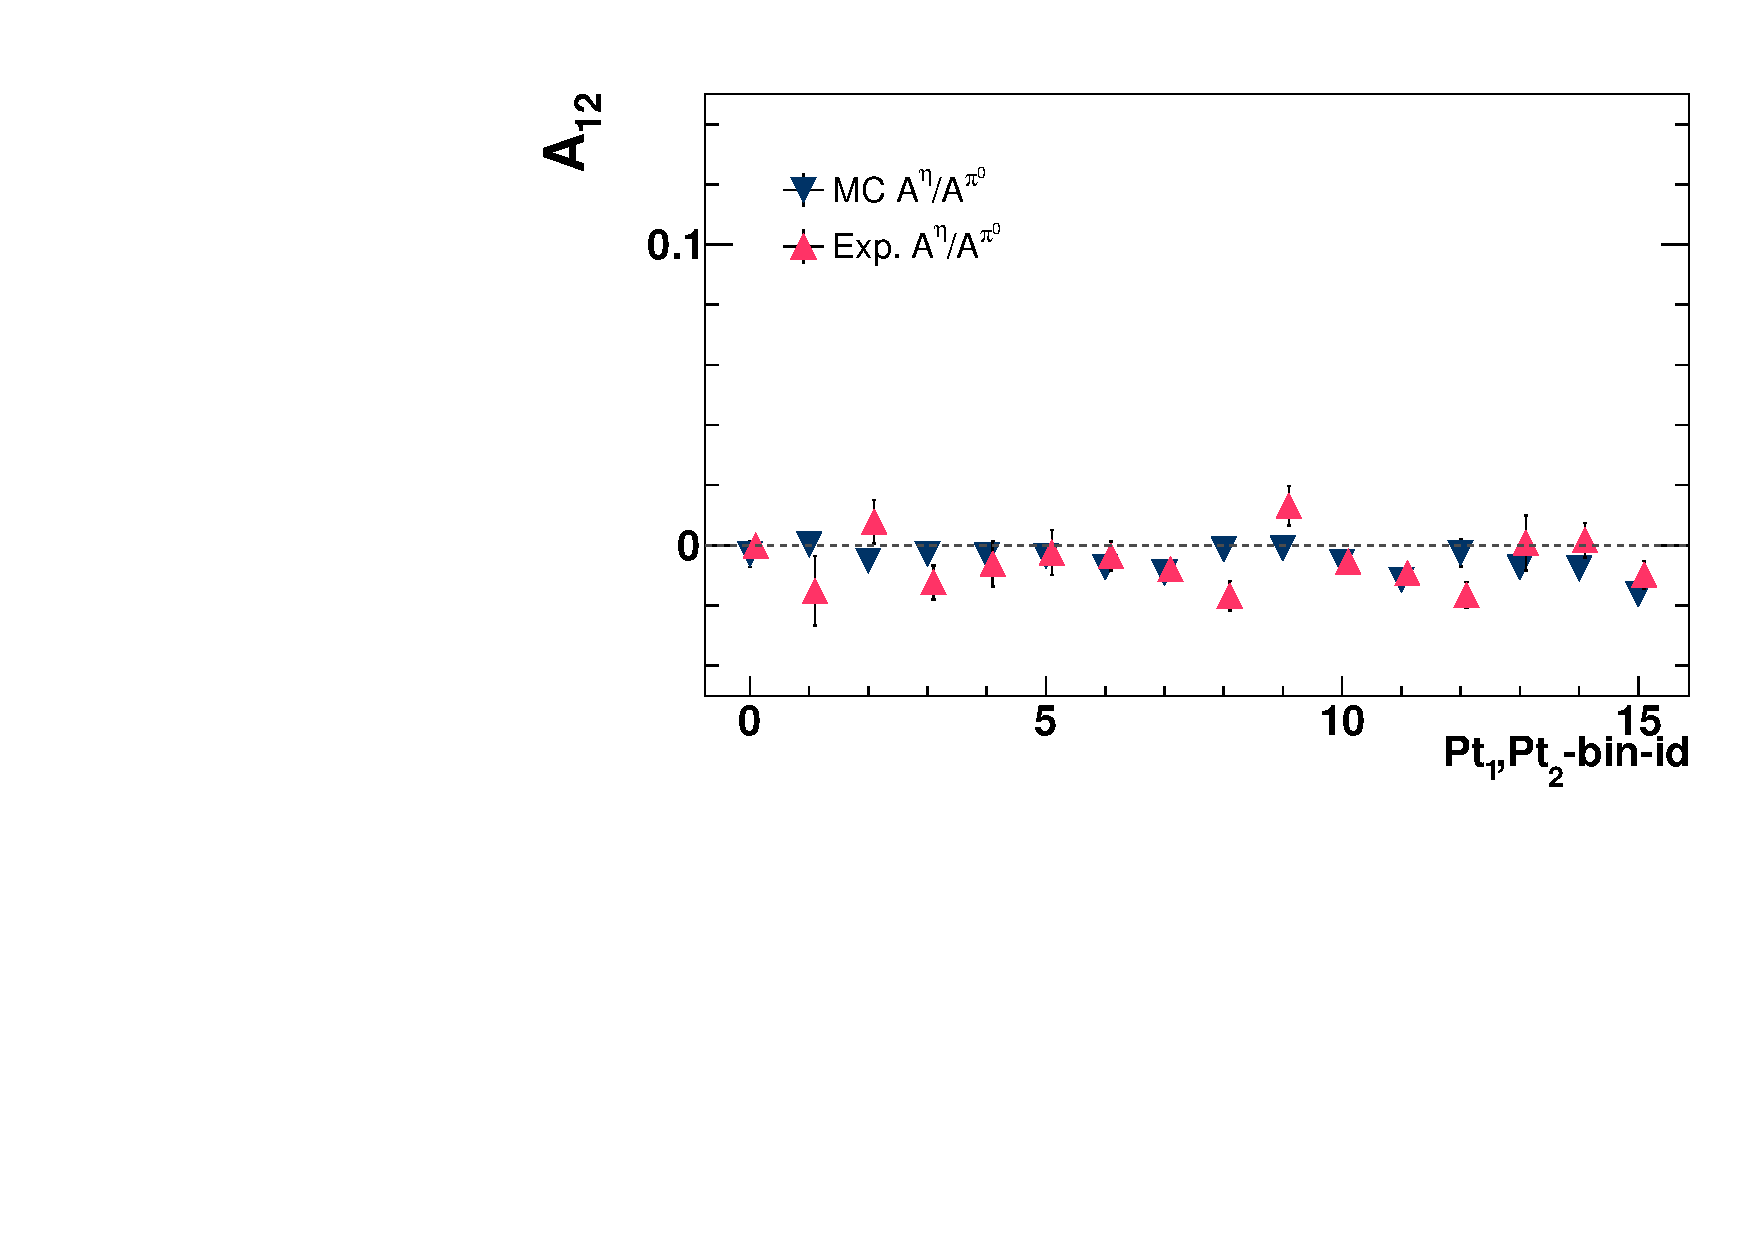
\includegraphics[width=.48\textwidth,natwidth=600,natheight=400]{figure_asy/Pi0OverEta3.pdf}}
  \caption[Asymmetry $\nicefrac{A^{0\pm}_{12}}{A^{\eta\pm}_{12}}$]{Asymmetry $\nicefrac{A^{0\pm}_{12}}{A^{\eta\pm}_{12}}$. Note that the legend in the plots is incorrect.}
  \label{fig:exp_pi0_eta_ratio}
\end{figure}
%As will be discussed in section~\ref{sec:comparewpreviouse}, there is an expectation that the UC double ratio written in Eqn.~\ref{eqn:chargeddoubleratio2} is comparable with $\pi^0$ double ratio~\ref{eqn:FF5}. This can be used to test for systematic effects by introducing a new double ratio:
%\begin{equation}
%\frac{A^{0\pm}_{12}}{A^C_{12}}=\frac{\pi^0\pi^++\pi^0\pi^-}{\pi^+\pi^++\pi^-\pi^++\pi^+\pi^-+\pi^-\pi^-}\\
%\end{equation}
%If detector effect is eliminated by fiducial cuts, the asymmetry of this new double ratio should be zero using both MC and experimental data. Figure~\ref{fig:exp_pi0_eta_ratio2} demonstrates the validity of our hypothesis and at the same time that the fiducial cuts together with the double ratio method eliminate false asymmetries. 
%\begin{figure}[H]
%  \centering     
 % \subfigure[$\pi^0$ double ratio over UC double ratio $z_1$ bins]{\label{fig:eta_singlez_ratio2}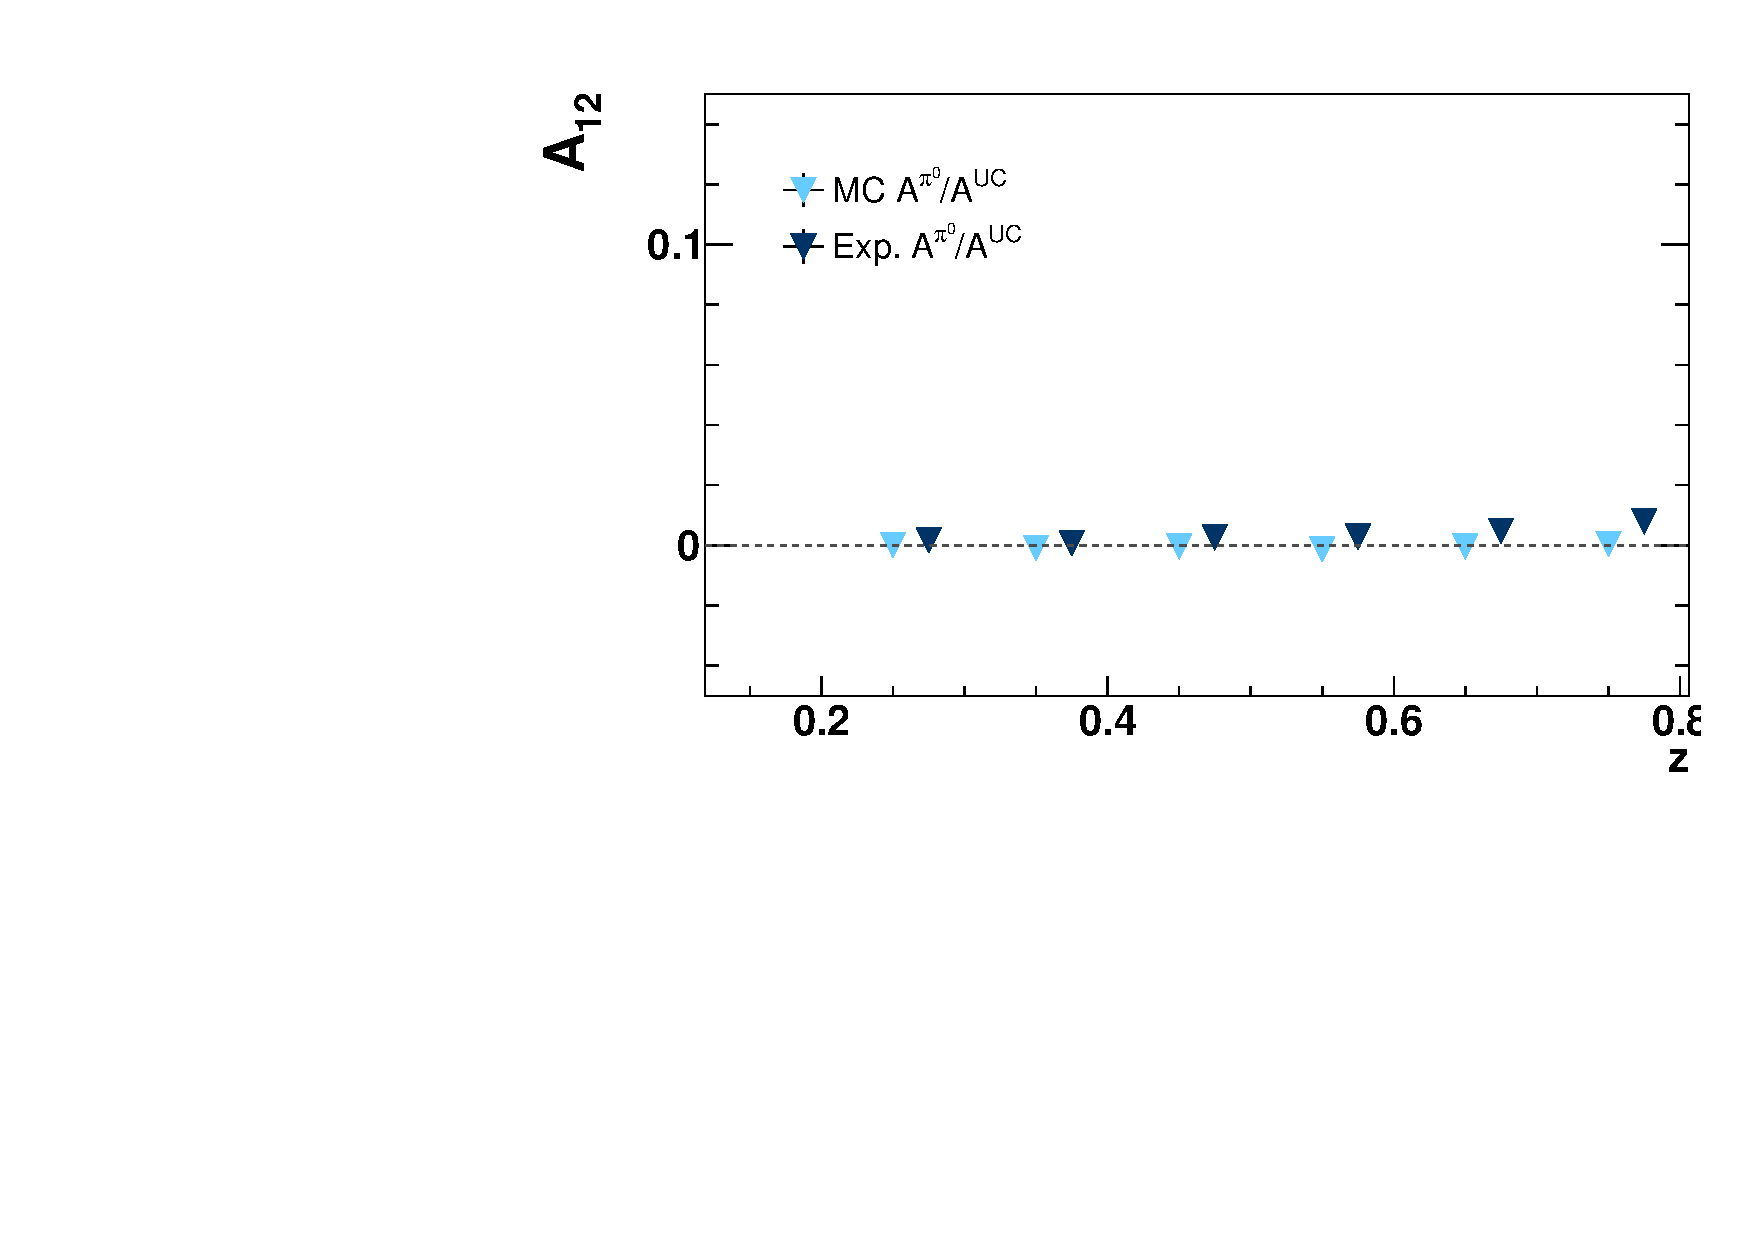
\includegraphics[width=.48\textwidth,natwidth=600,natheight=400]{figure_asy/Pi0OverUC0.pdf}}
  % \subfigure[$\pi^0$ double ratio over UC double ratio $P_{t1}$ bins]{\label{fig:exp_comz_ratio2}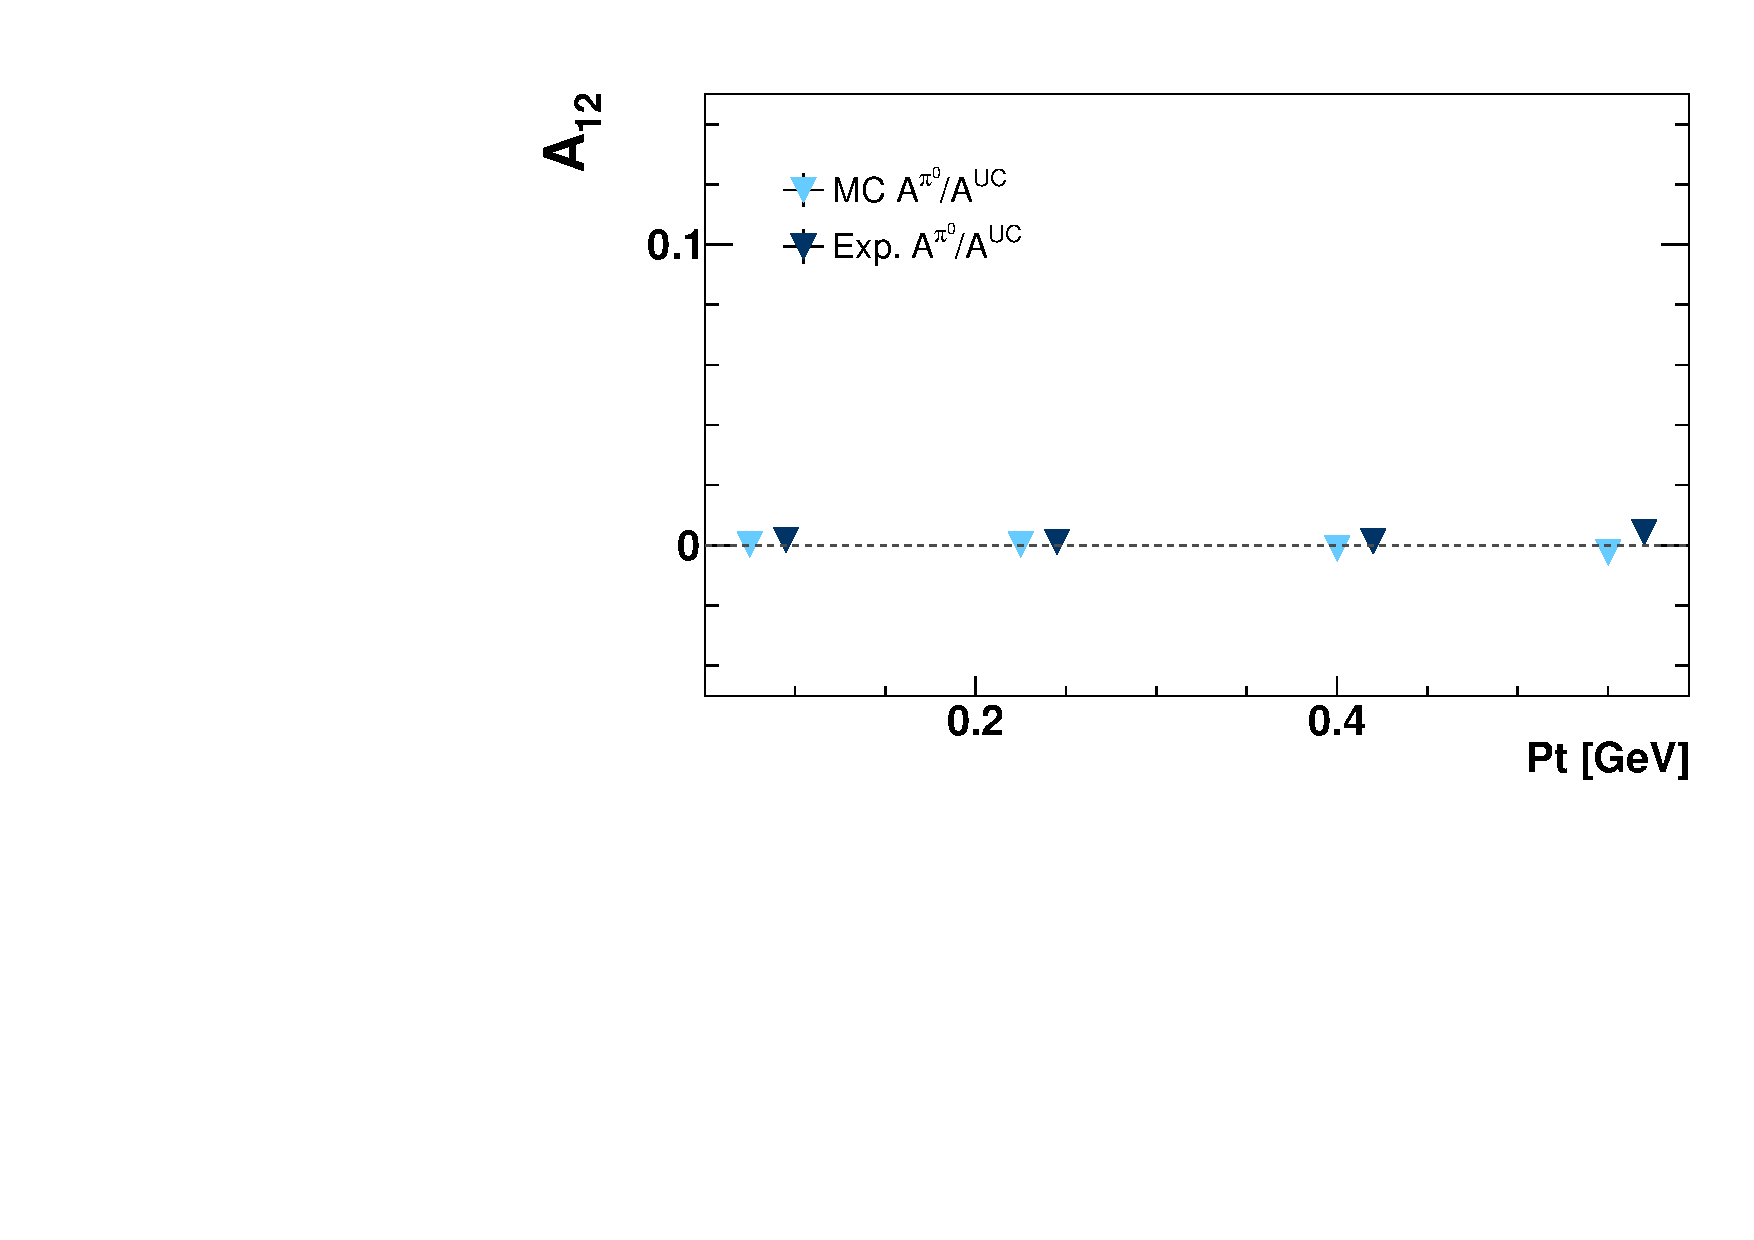
\includegraphics[width=.48\textwidth,natwidth=600,natheight=400]{figure_asy/Pi0OverUC2.pdf}}
 % \subfigure[$\pi^0$ double ratio over UC double ratio $(z_1,z_2)$ bins]{\label{fig:exp_signlept_ratio2}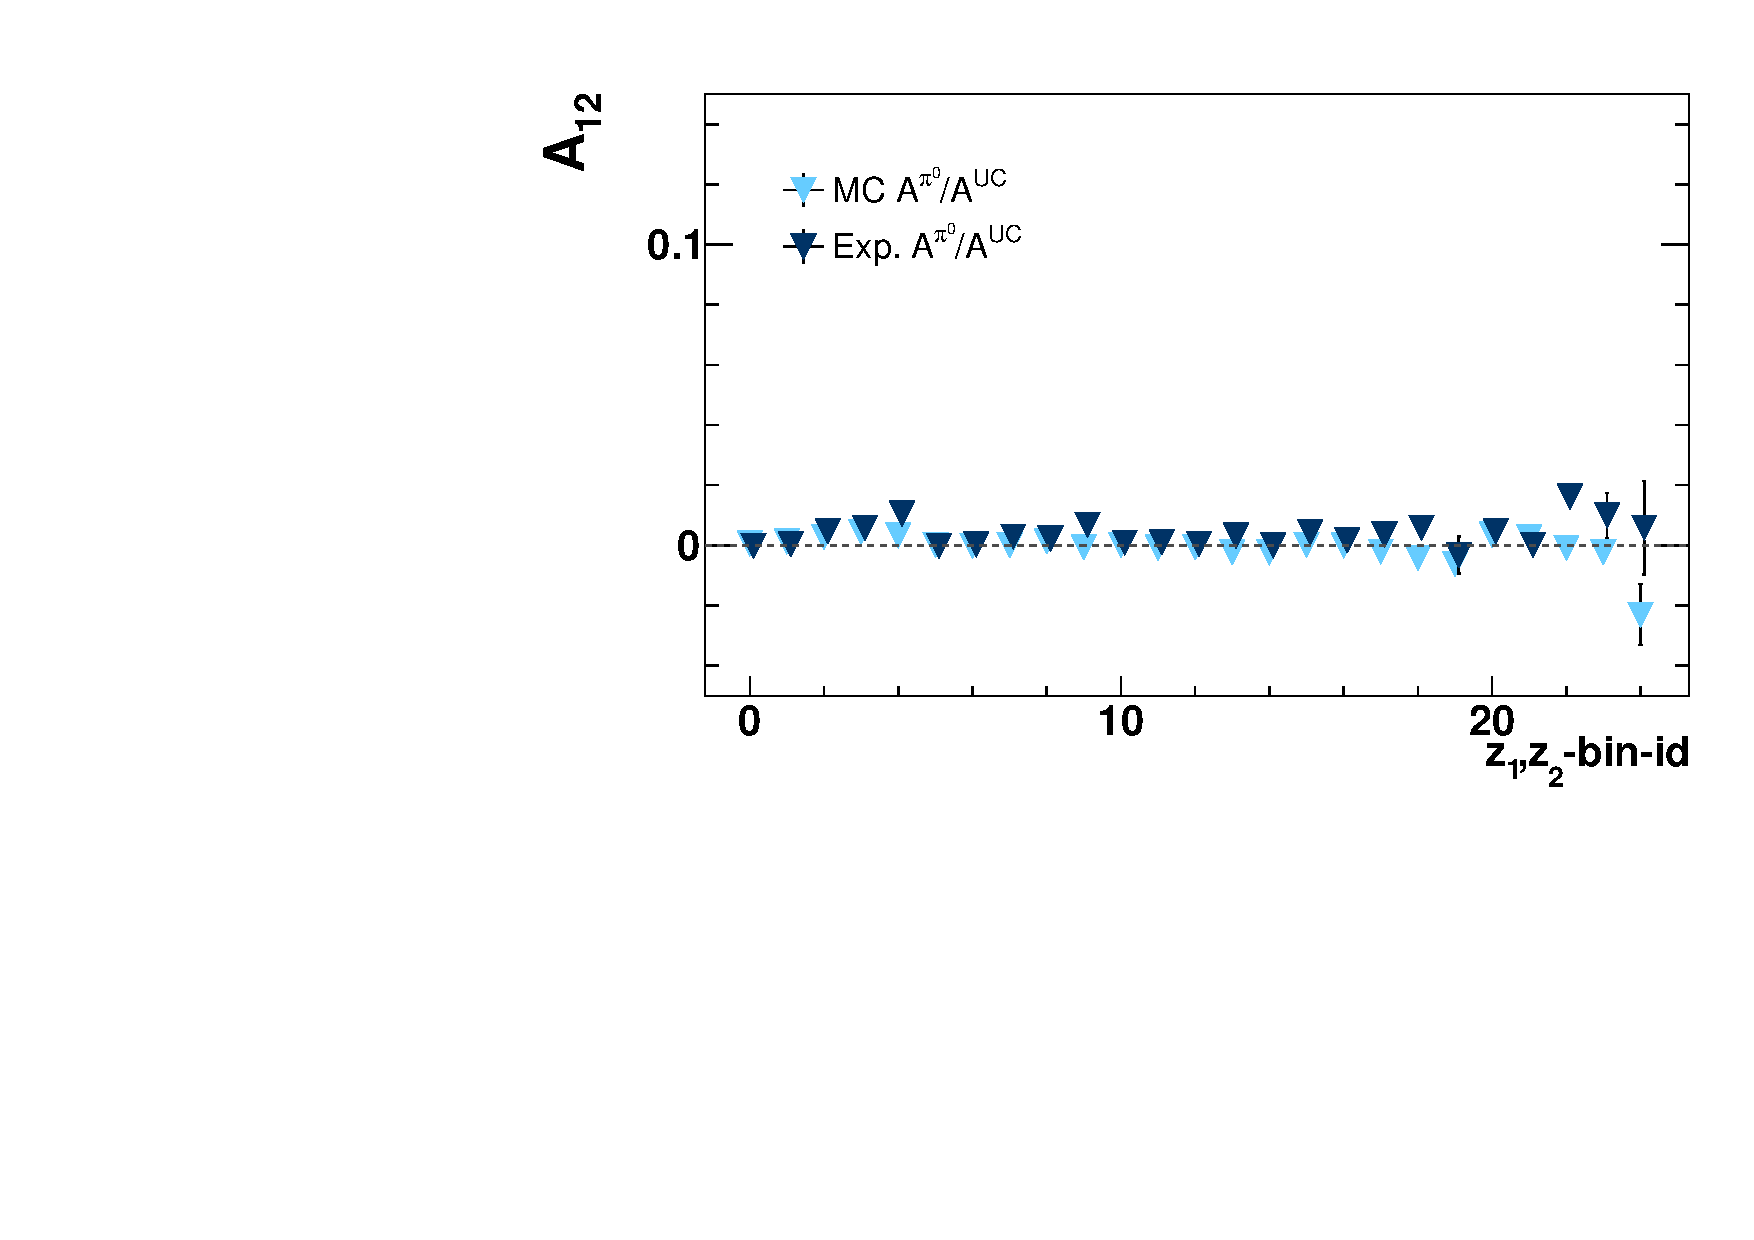
\includegraphics[width=.48\textwidth,natwidth=600,natheight=400]{figure_asy/Pi0OverUC1.pdf}}
 % \subfigure[$\pi^0$ double ratio over UC double ratio $(P_{t1},P_{t2})$ bins]{\label{fig:exp_compt_ratio2}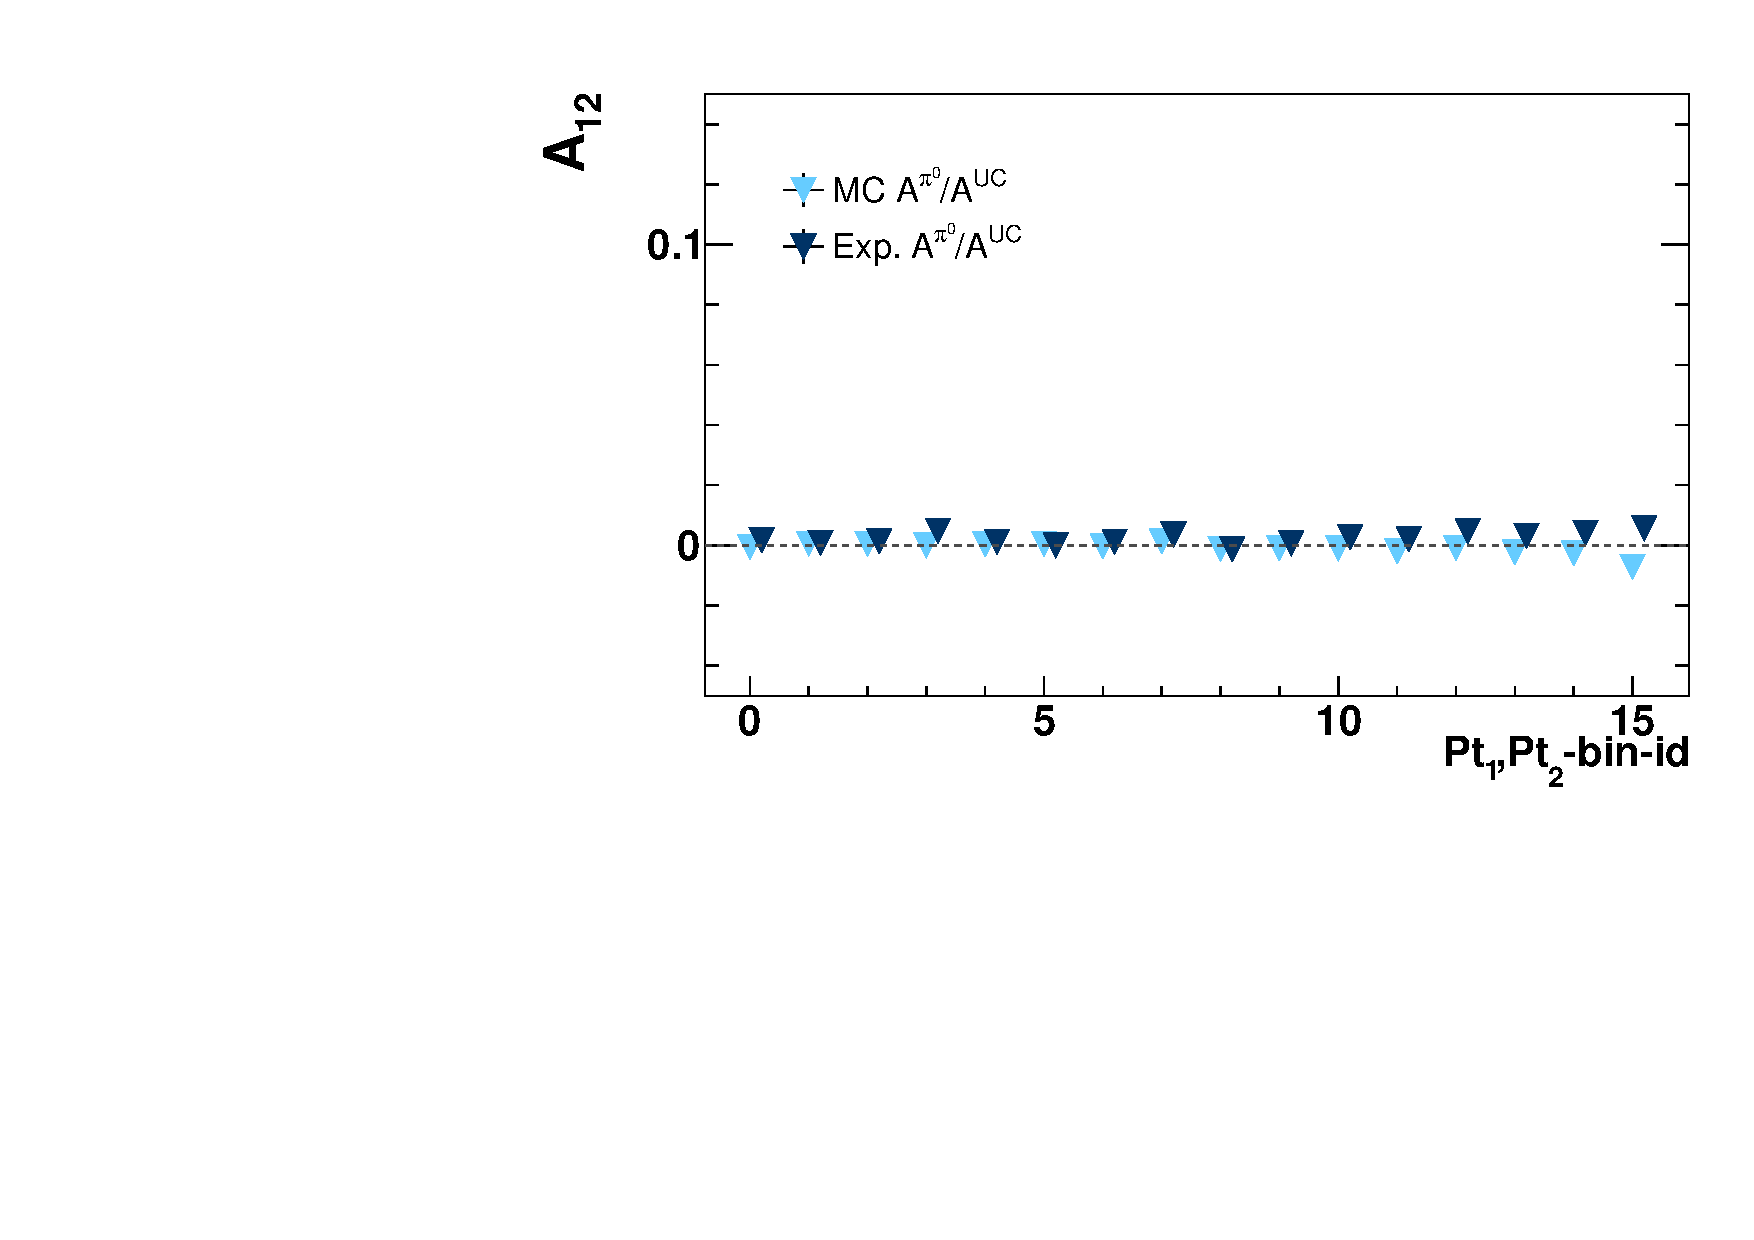
\includegraphics[width=.48\textwidth,natwidth=600,natheight=400]{figure_asy/Pi0OverUC3.pdf}}
  %\caption{Double ratio asymmetry $\nicefrac{A^{0\pm}_{12}}{A^C_{12}}$, the dark blue points are from experiment data and the light blue points are MC.}
  %\label{fig:exp_pi0_eta_ratio2}
%\end{figure}



